\documentclass[
    12pt,
    oneside,
    a4paper,
    english,
    brazil
]{abntex2}

\usepackage{lmodern}
\usepackage[T1]{fontenc}
\usepackage[utf8]{inputenc}
\usepackage{indentfirst}
\usepackage{color}
\usepackage{graphicx}
\usepackage{microtype}
\usepackage{amsfonts}
\usepackage{amsmath}
\usepackage{csquotes}
\usepackage{subcaption}
\usepackage[table]{xcolor}

\usepackage{tikz}
\usetikzlibrary{positioning}

\usepackage{caption}

\usepackage[brazilian,hyperpageref]{backref}
\usepackage[alf]{abntex2cite}

\usepackage{macros}

\titulo{Previsão de séries temporais por meio de aprendizado de máquina}
\autor{Guilherme Chichanoski}
\local{Maringá}
\data{2019}
\orientador{Valéria Delisandra Feltrim}
\instituicao{Universidade Estadual de Maringá\\
             Centro de Tecnologia --- Departamento de Informática\\
             Bacharelado em Ciência da Computação}
\tipotrabalho{Trabalho de Conclusão de Curso}

\preambulo{Trabalho  de   Conclusão  de  Curso  de   Graduação  apresentado  ao
    Departamento  de  Informática da  Universidade  Estadual  de Maringá,  como
    requisito  parcial  para  obtenção  do  grau  de  Bacharel  em  Ciência  da
    Computação.}

\makeatletter
\hypersetup{
    pdftitle={\@title},
    pdfauthor={\@author},
    pdfsubject={\imprimirpreambulo},
    pdfcreator={LaTeX with abnTeX2},
    pdfkeywords={séries temporais}{arima}{aprendizado de máquina}{redes neurais},
    colorlinks=true,   % false: boxed links; true: colored links
    linkcolor=red,     % color of internal links
    citecolor=green,   % color of links to bibliography
    filecolor=magenta, % color of file links
    urlcolor=blue,
    bookmarksdepth=4
}
\makeatother

\setlength{\parindent}{1.3cm}
\setlength{\parskip}{0.2cm}

\begin{document}

\frenchspacing

\imprimircapa{}

\imprimirfolhaderosto{}

\begin{epigrafe}
    \vspace*{\fill}
    \begin{flushright}
        \textit{``Rogo a você que me lê\\
        A sua boa vontade\\
        Não olhe os erros, releve,\\
        Guarde com sinceridade\\
        E busque o melhor fazer\\
        Lendo cordel de verdade.''\\
        Raquel Juvêncio e Filomena Mourão}
    \end{flushright}
\end{epigrafe}

\begin{resumo}

    Prever  eventos  em  séries  temporais  é uma  tarefa  muito  importante  e
    complexa,  para isso  muitos autores  utilizam-se de  métodos estatísticos,
    como  o ARIMA  para realizar  essas  previsões. No  entanto outros  métodos
    com  base em  aprendizado de  máquina, mais  especificamente redes  neurais
    artificiais, tem se demonstrado substitutos a altura. Foi utilizada a série
    S\&P500 para verificação do desempenho  dessas abordagens, e como resultado
    foi concluído  que para previsões de  um dia adiante a  utilização de redes
    neurais  artificiais  apresenta  um  desempenho  ligeiramente  inferior  ao
    ARIMA\@.

    \textbf{Palavras-chave}: séries temporais, arima, aprendizado de máquina,
    redes neurais.
\end{resumo}

\begin{resumo}[Abstract]
    \begin{otherlanguage*}{english}

    Predicting events  in time  series is  a very  important and  complex task,
    for  which many  authors  use statistical  methods such  as  ARIMA to  make
    these predictions.  However other methods  based on machine  learning, more
    specifically artificial  neural networks,  have obtained good  results. The
    S\&P500 series was used to verify  the performance of these approaches, and
    as  a  result it  was  concluded  that for  one-day  forecasts  the use  of
    artificial  neural  networks presents  a  slightly  lower performance  than
    ARIMA\@.

    \textbf{Keywords}: time series, arima, machine learning, neural
    networks.
    \end{otherlanguage*}
\end{resumo}

\textual{}

\pdfbookmark[0]{\contentsname}{toc}
\tableofcontents*
\cleardoublepage{}

\chapter{Introdução}

%VALERIA: Evite usar a 1a pessoa no texto ("podemos..., fizemos...", etc.). Embora essa forma seja comum na escrita científica em inglês, em português não é usual. Eu já corrigi essa questão em toda a parte revisada (até o início dos modelos probabilísticos). Por favor, corrija no restante.

Segundo \citeonline{wiley} prever é a capacidade de predizer valores ou eventos
futuros e  constitui uma  tarefa de grande  importância para  diversos setores,
incluindo governos e indústrias. Uma vez  que tal capacidade é parte crucial na
tomada de decisão,  fica evidente a necessidade de se  realizar boas previsões.
No entanto,  fazer boas  previsões pode ser  uma tarefa  extremamente complexa.
Muitos autores  e organizações já realizaram  previsões que, com o  decorrer do
tempo, se mostraram erradas, como no caso  do The New York Times, que previu em
1966  que existiriam  somente 220 000  computadores nos  Estados Unidos  no ano
2000.

Ainda conforme  \citeonline{wiley}, as  previsões são classificadas  como sendo
de  curto,  médio  e  longo  prazo,   sendo  o  prazo  definido  na  frequência
das  observações.  Quando denominadas  de  curto  prazo, são  previstas  poucas
observações  a frente  do tempo  atual. Já  previsões de  médio prazo  podem se
estender por algumas observações no futuro.  Por fim, previsões que envolvem um
período maior  no futuro são chamadas  de longo prazo. Ainda  conforme o autor,
predições de médio e longo prazo são mais difíceis de se realizar e suscetíveis
a fatores externos.

Para a realização da previsão é necessária  a compreensão do evento que se quer
prever. Quando  existe uma relação temporal  entre as observações do  evento em
questão,  i.e., o  evento  ocorre  em uma  determinada  sequência  no tempo,  é
necessário organizar  as informações  de forma a  evidenciar a  dependência das
observações com  seus estados anteriores.  Nesse caso, as  observações passadas
compõem uma  série temporal, a  partir da qual  é possível realizar  medições e
produzir modelos capazes de expressar  matematicamente o comportamento da série
em  função de  suas  observações  anteriores, permitindo  assim  a predição  de
estados futuros.

Conforme  mencionado,   as  séries  temporais  são   compostas  de  observações
sequenciais ao  longo do  tempo~\cite{wiley}. Como exemplo,  a \autoref{serie0}
mostra uma série gerada utilizando-se um processo de caminhada aleatória. Sendo
essas observações  separadas unicamente pelo  tempo, pode-se obter os  dados em
diferentes intervalos,  como observações diárias, semanais  ou anuais. Conforme
\citeonline{ehlers},  devido  à  caraterística  estocástica  do  processo,  uma
observação se define em função de suas antecessoras.

\begin{figure}[ht]
    \centering
    \caption{Série gerada para exemplo}\label{serie0}
    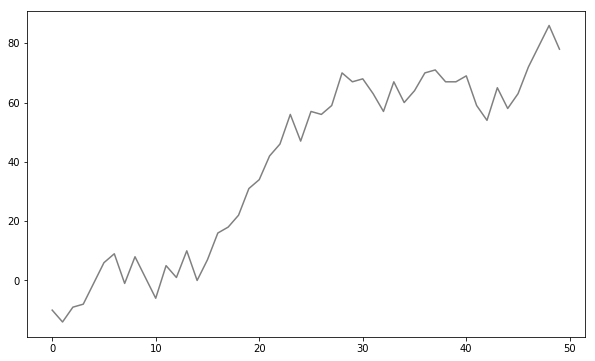
\includegraphics[width=.5\linewidth]{images/serie_exemplo.png}
    \source{Elaborado pelo autor}
\end{figure}

Considerando  então  que  a  série  apresentará  comportamento  estocástico,  é
possível  propor  modelos  que  serão  capazes  de  aproximar  o  comportamento
da  série.  Os  modelos  comumente  utilizados para  essa  tarefa  são  aqueles
probabilísticos, mais especificamente o ARIMA\@, proposto por \citeonline{box}.
Também é possível utilizar modelos criados a partir da aplicação de técnicas de
aprendizado de máquina,  que vem se apresentando como  uma alternativa poderosa
em muitas aplicações.

Com o  constante interesse na  aplicação e  a identificação das  capacidades de
técnicas de  aprendizado, fica  evidente a importância  de observar  como esses
modelos se comparam com os estatísticos. Dessa forma, o objetivo deste trabalho
foi comparar o desempenho de modelos  estatísticos e baseados em aprendizado de
máquina na previsão de uma  série de característica econômica. Especificamente,
foram  avaliados  o  modelo  estatístico  ARIMA  e  um  modelo  de  aprendizado
de  máquina baseado  em  redes  neurais artificiais  de  múltiplas camadas.  Os
resultados indicaram que  os modelos tiveram desempenhos  semelhantes nos dados
utilizados nesse trabalho.

% Como  forma de  comparar desempenhos  e  buscar compreender  as técnicas  que
% poderiam ser utilizadas para a previsão, este trabalho realizou a previsão de
% uma série de característica econômica utilizando ambas metodologias.

% TODO: Introduzir modelos ARIMA com exemplos de artigos

% FIXME Mais adequado na parte de trabalhos relacionados
%vez mais  notórias pelos bons resultados  que oferecem. \citeonline{artigoEx3}
%Em contrapartida, técnicas  de aprendizado de máquinas estão  se tornando cada
%aplicou  métodos  de aprendizado  de  máquina  possibilitando a  previsão  com
%bons  resultados. Pelo  fato  dos modelos  estatísticos fornecerem  resultados
%satisfatórios para predições e estarem bem difundidos na comunidade acadêmica,
%é  comum  que  trabalhos  como \citeonline{artigoEx4}  compare  os  resultados
%obtidos  a  partir  de  aprendizado   de  máquina  com  modelos  de  abordagem
%estatísticas. Para modelos de aprendizado se  destaca aqueles com uso de redes
%neurais  artificiais  por serem  capazes  de  obter bons  resultados  conforme
%analisado  por \citeonline{zhang},  o  autor ainda  apresenta outros  exemplos
%quais os autores obtiveram resultados superiores ao método estatístico.

O    restante   desta    monografia    está   organizada    como   segue.    No
\autoref{chap:fundTeor}  é apresentada  a  fundamentação  teórica do  trabalho,
incluindo os  principais métodos  de previsão  de séries  temporais empregados.
No  \autoref{chap:trab_relacionados} foram  apresentados  outros trabalhos  que
abordam  o   tema.  Já  no   \autoref{chap:desenv}  são  descritos   os  passos
metodológicos  empregados para  a desenvolvimento  tanto do  modelo estatístico
quanto  de  aprendizado  de  máquina.   Os  resultados  obtidos  com  base  nos
modelos construídos são apresentados  no \autoref{chap:result} e apresentada as
constatações  feitas  em ambos  modelos.  Por  fim, no  \autoref{chap:concl}  é
apresentada a conclusão do que foi realizado.

\chapter{Fundamentação teórica}\label{chap:fundTeor}

\section{Previsão}
Segundo  \citeonline{wiley},  o  processo  de previsão  pode  ser  dividido  em
diversas atividades, dispostas a seguir:

\begin{enumerate}
    \item Definição do problema\\
        Envolve  definir e  entender  a  tarefa de  previsão  a ser  realizada,
        considerando o prazo a ser previsto e definindo os dados necessários.
    \item Coleta dos dados\\
        Envolve a coleta  dos dados necessários de acordo com  as definições da
        atividade anterior.
    \item Análise dos dados\\
        Atividade de alta  importância para a seleção do  modelo mais adequado.
        Nessa  etapa   são  utilizadas  observações  gráficas   e  extração  de
        características para identificar padrões  que corroborem na escolha dos
        parâmetros. Também são identificadas  observações problemáticas e, caso
        necessário, aplicadas as devidas correções.
    \item Seleção e verificação do modelo\\
        A partir  da análise  feita na atividade  anterior, será  selecionado o
        modelo, analisando-se  também o comportamento com  os dados fornecidos.
        Como  método de  verificação são  utilizadas métricas  que favoreçam  a
        comparação.
    \item Avaliação do modelo\\
        Atividade na qual se avalia como  o modelo se comporta com novos dados,
        normalmente realizada  com observações  excluídas dos  dados utilizados
        nas atividades anteriores. As  observações separadas para avaliação são
        utilizadas apenas para essa finalidade.
    \item Publicação do modelo\\
        Com o modelo devidamente selecionado e avaliado, o mesmo é instalado em
        ambiente de produção, observando-se  as alterações necessárias para que
        novos dados sejam inseridos corretamente.
    \item Monitoramento do desempenho do modelo\\
        Deve-se continuamente  avaliar como  o modelo  aplicado se  comporta em
        relação ao ambiente, já que o ambiente é algo volátil.
\end{enumerate}

Essas  atividades  normalmente  são  realizadas em  ordem  como  exposta.  Vale
observar  ainda  que   se  os  resultados  da  atividade   de  avaliação  forem
insatisfatórios, deve-se  retornar à atividade  anterior e refazer  a avaliação
até que um modelo que obedeça às especificações seja encontrado.

\section{Séries temporais}\label{sec:seriesTemporais}

Como  exposto anteriormente,  séries  temporais são  compostas por  observações
sucessivas  feitas ao  longo do  tempo. Cabe  destacar ainda  que essas  séries
se  caracterizam   pelo  fato  de   suas  observações  serem   dependentes  das
observações  anteriores. Além  disso,  tais  séries demonstram  características
como  tendência e  sazonalidade.  A tendência  caracteriza  o comportamento  de
crescimento/decrescimento da série, o que  pode levar a observações futuras com
valores  menores ou  maiores. A  sazonalidade caracteriza  padrões cíclicos  em
função do tempo, comumente tomando períodos semanais, mensais ou anuais.

Uma série é descrita matematicamente pelo conjunto $\{X(t): t \in T\}$, podendo
$t$ ser  um tempo  contínuo ou  discreto. O  tempo $t$  é dito  contínuo quando
se  possui  observações  $X(t)$  para  todo $t$  em  $T$,  sendo  $T  \subseteq
\mathbb{R}^{+}$. O tempo $t$ é discreto  quando entre as observações $X(t_i)$ e
$X(t_{i+1})$ existe um  intervalo igual de tempo, normalmente dado  na forma de
uma sequência, $T = \{1, 2, \ldots, n\}$, sendo $n$ o número de observações.

Segundo  \citeonline{ehlers}, uma  série  temporal  classicamente é  decomposta
seguindo a \autoref{eq:timeseries}, sendo $t$ usado para denotar o tempo, logo,
é parte fundamental entender o comportamento segundo essas três componentes.

\begin{equation}
    \label{eq:timeseries}
    X_t = Tendência_t + Sazonal_t + Aleatório_t
\end{equation}

\subsection{Série estacionária}\label{sec:estacionaria}

Um  conceito   importante  para  a  análise   de  séries  temporais  é   o  seu
caráter  estacionário.  Um  processo  é  dito estacionário  se  todas  as  suas
características  comportamentais não  se  alteram ao  longo  do tempo.  Segundo
\citeonline{timeseriesExample} não existe  um limiar que defina  uma série como
estacionária, mas pode  definir como estacionário um processo  se desenvolve no
tempo em  torno da média, de  modo que a escolha  de uma origem dos  tempos não
é  importante.  Segundo  \citeonline{ehlers},  uma série  é  dita  estritamente
estacionária  quando  a  distribuição  de probabilidade  conjunta  de  $X(t_1),
\ldots, X(t_k)$ é igual a de $X(t_1 + \tau), \ldots, X(t_k + \tau)$.

Ainda segundo \citeonline{ehlers}, a definição  estrita de série estacionária é
dificilmente  aplicada,  então  usualmente  se utiliza  a  definição  de  série
fracamente estacionária,  que se define com  base no critério da  mesma possuir
função média constante. Dessa forma,  neste trabalho, foi utilizada a definição
de série fracamente estacionária para se tomar uma série como estacionária.

Em  termos matemáticos,  usa-se a  \autoref{eq:westacionaria} para  definir que
variância  de um  elemento da  série ($z_t$)  deve ser  semelhante à  média. Em
outras  palavras, o  deslocamento da  origem do  tempo $t$  por uma  quantidade
$\tau$ não  exerce efeito  na distribuição  conjunta da  série. Assim,  o valor
esperado para a série em determinado momento não será dada em função do tempo.

\begin{equation}
    \label{eq:westacionaria}
    E(z_t) = \mu_t = \mu
\end{equation}

% FIXME Dada em função de que??


%TODO Adicionar referência ao Livro Time Series by exmples

%TODO Adicionar referência ao teste de Dockey Fuller

% VALERIA: Deixe para mostrar o exemplo da série estacionária pós-diferenciação
% na seção que fala  sobre a diferenciação. Neste ponto do  texto ficou fora de
% contexto. Ou, se  vc quer mostrar um exemplo, mostre  uma série originalmente
% estacionária. Além  disso, nesse caso, vc  tem que explicar melhor  a figura.
% Por exemplo,  qual(is) característica(s) do  gráfico da série me  diz(em) que
% ela é  estacionária? Dizer  que a  observação do gráfico  é suficiente  não é
% suficiente. ;)

Segundo  \citeonline{timeseriesExample} embora existam testes  como o  de Dikey
Fuller  descrito  em  \citeonline{dickey}  para a  prova  de  estacionariedade,
é  suficiente  a observação  gráfica  da  série.  Caso  não seja  conclusiva  a
observação \citeonline{timeseriesExample} orienta obter  o gráfico da função de
autocorrelação,  e  se  observada  a  existência  de  mais  de  20  correlações
significativas pode-se classificar a série como não estacionária.

\subsection{Sazonalidade e tendência}

Conforme   definido  por   \citeonline{ehlers},   a  sazonalidade   caracteriza
repetições  de comportamento  de uma  série em  um período  $s$. A  presença da
sazonalidade,  em geral,  é facilmente  observada na  representação gráfica  da
série, conforme exemplificado no gráfico  da \autoref{fig:co2}. Nesse gráfico é
apresentada uma série  temporal real que registra a mudança  na concentração de
$CO_2$ na atmosfera. Observando o gráfico, é possível notar que há sazonalidade
de periodicidade anual, devido ao gráfico apresentar formato de serra e este se
apresentar em repetição anual.

Ainda  no  gráfico  da  \autoref{fig:co2},  também  é  possível  notar  que  há
uma  tendência de  crescimento na  série. Segundo  \citeonline{ehlers}, não  há
uma  definição exata  de  tendência, mas, normalmente, a  mesma é associada  ao
comportamento  de  mudança  das  observações  ao longo  de  um  vasto  período.
Uma  série  com tendência  pode  ser  descrita  como  a função  apresentada  na
\autoref{eq:tendencia},  na  qual $\alpha$  e  $\beta$  são os  coeficientes  e
$\epsilon_t$ é um erro aleatório  de distribuição normal. O coeficiente $\beta$
define a taxa de  crescimento da série, podendo ser dado  como um função global
ou definido localmente.

\begin{equation}
    \label{eq:tendencia} X_t = \alpha + \beta{}t + \epsilon_t
\end{equation}

% Um exemplo real de uma série  temporal que apresenta tendência e sazonalidade
% é mostrado  no gráfico  na \autoref{fig:co2}. Essa  série registra  a mudança
% na  concentração  de $CO_2$  na  atmosfera,  sendo,  portanto, uma  série  de
% característica natural.  Observando o gráfico,  é fácil notar a  tendência de
% crescimento da série e sua sazonalidade de periodicidade anual.

\begin{figure}[ht]
    \centering
    \caption{Leituras de $CO_2$ na atmosfera.}\label{fig:co2}
    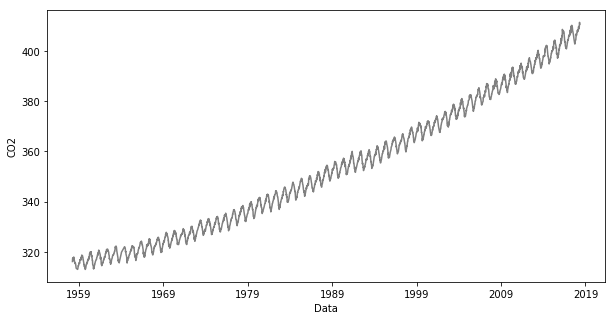
\includegraphics[width=.5\linewidth]{images/co2.png}
    \source{\citeonline{co2data}}
\end{figure}

\subsubsection{Filtros}

Em  algumas séries, a  tendência pode  não estar  evidente  devido ao  processo
aleatório. Por conta disso, pode ser  necessária a aplicação de filtros que têm
como objetivo obter  uma série suavizada que possibilite  observar a tendência.
Um desses filtros é apresentado na \autoref{eq:filtro}~\cite{ehlers}.

\begin{equation}
    \label{eq:filtro}
    y_t = \sum_{j = -q}^{s}{a_{j}x_{t+j}}
\end{equation}

Na \autoref{eq:filtro}, $a_j$  é um coeficiente a ser aplicado  a cada termo da
soma de forma a aplicar um peso a este, sendo observado que $\sum{a_j} = 1$.

A  \autoref{eq:yjfiltro}  é  conhecida  por   fornecer  o  cálculo  das  médias
móveis,  permitindo  suavizar  a  série,  mantendo  a  tendência.  A  aplicação
do  filtro  de médias  móveis  nos  dados das  leituras  de  $CO_2$ resulta  na
\autoref{fig:co2filtrado}.  Esta evidencia  de forma  independente a  tendência
após  a  remoção  da  sazonalidade,  por meio  da  suavização  utilizando  como
parâmetro $q$ seu período cíclico.

\begin{equation}
    \label{eq:yjfiltro}
    y_t = \frac{1}{2q + 1}\sum_{j=-q}^{q}{x_{t+j}}
\end{equation}

\begin{figure}[ht]
    \centering
    \caption{Leituras de $CO_2$ filtrada utilizando médias móveis com $q$ igual
        a $52$, devido à sazonalidade ser anual, ou seja, $52$
        semanas.}\label{fig:co2filtrado}
    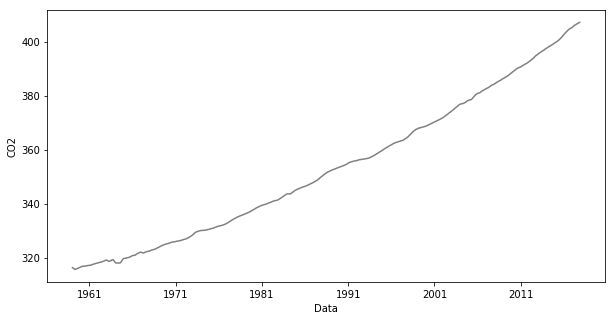
\includegraphics[width=.5\linewidth]{images/co2_filtered.png}
    \source{Elaborado pelo próprio autor a partir de \citeonline{co2data}}
\end{figure}

\subsubsection{Diferenciação}\label{sec:diff}

Outra tarefa a ser observada em relação  ao entendimento de tendência é a forma
na qual é removida. O método mais  simples para remoção da tendência é subtrair
de  cada valor  observado  o  valor do  seu  antecessor,  conforme descrito  na
\autoref{eq:diferenciacao}. Normalmente,  uma única diferenciação  é suficiente
para remover  a tendência, porém em  séries com componente sazonal  podem vir a
ser necessárias mais de uma em um \textit{lag} diferente.

\begin{equation}
    \label{eq:diferenciacao}
    y_t = x_t - x_{t-1}
\end{equation}

O gráfico  da \autoref{fig:co2diff} mostra o  resultado obtido para a  série de
leituras de $CO_2$ após uma diferenciação. Pelo gráfico é possível perceber que
a série resultante  se aproxima de uma série com  função média constante, dando
evidência a componente sazonal já que  a variação do gráfico apresenta um forte
comportamento repetitivo.

\begin{figure}[ht]
    \centering
    \caption{Série da leitura do $CO_2$ na atmosfera com uma
        diferenciação}\label{fig:co2diff}
    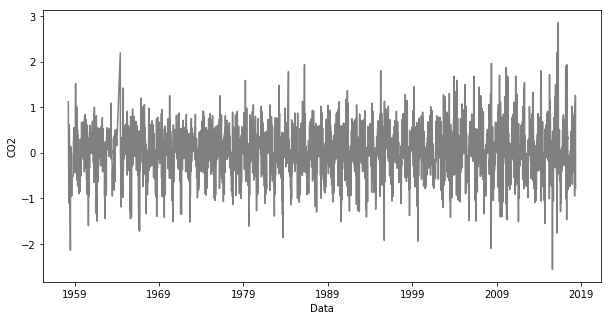
\includegraphics[width=.5\linewidth]{images/co2_diff.png}
    \source{Elaborado pelo autor a partir de \citeonline{co2data}}
\end{figure}

\section{Modelos probabilísticos}

Conforme  apresentado anteriormente,  as séries  temporais podem  ser previstas
utilizando-se modelos  estatísticos. Segundo \citeonline{ehlers}, isso  se deve
ao  seu caráter  estocástico, uma  vez  que cada  observação possui  correlação
com  as  observações  imediatamente   antecessoras,  diferentemente  de  séries
determinísticas, as quais têm seu estado  definido por uma função matemática ou
um sistema para o qual a saída é dependente apenas das entradas atuais.

Um modelo comumente utilizado para a  previsão de séries temporais é o ARIMA\@.
Descrito por  \citeonline{box}, esse  modelo caracteriza a  série em  termos de
três  parâmetros $(p,d,q)$,  sendo  cada  um associado  a  um  processo: $p$  é
associado a processos  autorregressivos, $d$ a integração e $q$  a processos de
médias móveis, embora de mesmo nome  este não tem qualquer associação ao filtro
de medias moveis.

A   definição  dos   valores   desses  parâmetros   depende   da  análise   das
características da  série. \citeonline{box}  descreveu algumas  ferramentas que
podem auxiliar nessa análise, entre elas a análise da função de autocorrelação.

\subsection{Função de autocorrelação}\label{sec:corre}

Como  o nome  sugere, a  função de  autocorrelação mede  a correlação  entre as
observações  de uma  série em  diferentes períodos.  Considerando-se uma  série
temporal $X$, calcula-se  a correlação entre seus valores com  uma defasagem de
tempo $k$,  sendo essa defasagem  a distância entre  o valor analisado  $X_t$ a
observação  $X_{t-k}$.  Por exemplo,  supondo  uma  série de  100  observações,
pode-se chamar de $X'$ a série  correspondente às 99 primeiras observações e de
$X''$ a série correspondente às últimas  99 observações. Nesse caso, tem-se uma
defasagem (ou \textit{lag}) de 1 período. Assim a função de autocorrelação será
dada segundo a \autoref{eq:autocorrelacao}.

\begin{equation}
    \label{eq:autocorrelacao}
    r_k = \frac{\sum_{t=1}^{n-k}{(x_t - \overline{x})(x_{t+k} -
    \overline{x})}}{\sum_{t=1}^{n}{(x_t - \overline{x})^2}}
\end{equation}

Segundo  \citeonline{ehlers},  a  função   de  autocorrelação,  quando  plotada
para  os  $k$-ésimos  primeiros  coeficientes,  é  chamada  de  correlograma  e
constitui-se em uma ferramenta importante para  as análises. Como um exemplo, a
\autoref{fig:correlogramaCo2}  apresenta o  correlograma  com  as 25  primeiras
defasagens das leituras de concentração  de $CO_2$ na atmosfera. Nesse gráfico,
também é exibido o intervalo de confiança de 95\% calculado para o correlograma
(destacado em  azul). Segundo \citeonline{ehlers},  o intervalo de  confiança é
necessário para se  definir quais correlações são relevantes e  quais não, pois
todas as  correlações importantes ficam  fora do intervalo de  confiança. Sendo
assim,  quando todas  as  correlações  estão dentro  do  intervalo,  a série  é
caracterizada  como  um ruído  branco,  ou  seja,  seu comportamento  não  pode
ser  modelado.  Para  encontrar  o  intervalo  de  confiança  do  correlograma,
\citeonline{ehlers} recomenda utilizar a equação $\pm{}2/\sqrt{n}$, sendo $n$ o
número de observações da série.

\begin{figure}[ht]
    \centering
    \caption{Gráfico da função de autocorrelação das leituras de
        $CO_2$}\label{fig:correlogramaCo2}
    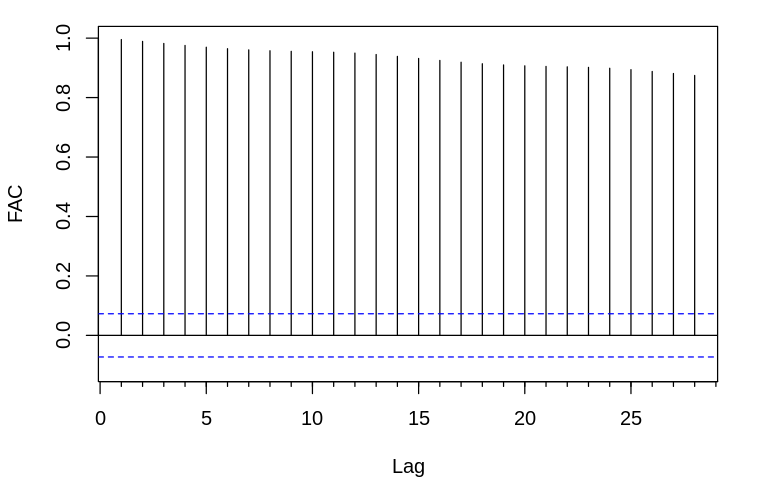
\includegraphics[width=.5\linewidth]{images/acf_co2.png}
    \source{Elaborado pelo autor a partir de \citeonline{co2data}}
\end{figure}

Para  exemplificar  como a  função  de  autocorrelação  pode ser  utilizada  na
definição do modelo estatístico, a  \autoref{fig:acfco2diff} mostra a função de
autocorrelação para a primeira diferenciação da série de leituras de $CO_2$. Se
observa que,  após diferenciada e removida  a tendência, é possível  observar o
comportamento sazonal, já que a  função de autocorrelação apresenta correlações
positivas e  negativas em uma distância  que pode ser entendida  como o período
cíclico da série.

\begin{figure}[ht]
    \centering
    \caption{Gráfico de função de autocorrelação da diferenciação da série de
        $CO_2$}\label{fig:acfco2diff}
    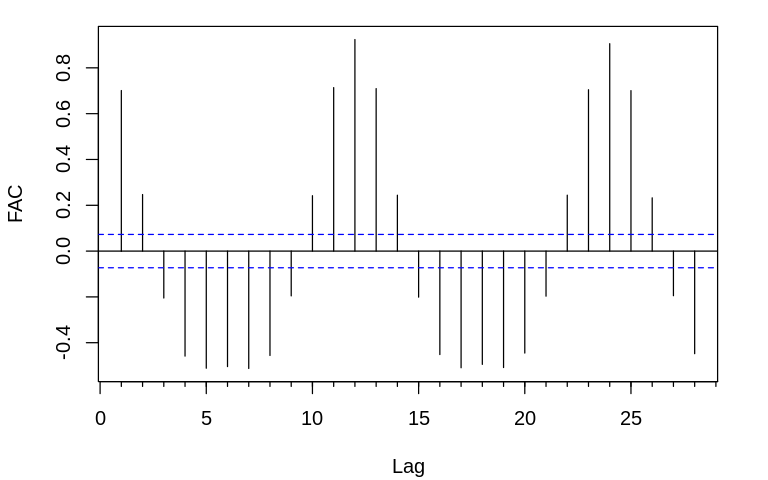
\includegraphics[width=.5\linewidth]{images/acf_co2_diff.png}
    \source{Elaborado pelo autor a partir de \citeonline{co2data}}
\end{figure}

\subsubsection{Função de autocorrelação parcial}

Durante a  análise, outra função relevante  é a de autocorrelação  parcial. Sua
definição, segundo  \citeonline{cryer}, é dada pela  \autoref{eq:facp}, na qual
$r_k$ é a autocorrelação da série $X$ no \textit{lag} $k$ e $\phi_{k,j}$ é dado
por $\phi_{k-1, j}-\phi_{kk}\phi_{k-1,k-j}$.

\begin{equation}
    \label{eq:facp}
    \phi_{kk} = \frac{r_k-\sum_{j=1}^{k-1}{\phi_{k-1,j}r_{k-j}}}{1-\sum_{j=1}^{k-1}{\phi_{k-1,j}r_{j}}}
\end{equation}

\subsection{ARIMA}

O  modelo ARIMA,  já  introduzido  na seção  anterior,  possui três  parâmetros
essenciais  $(p,q,d)$.  Segundo \citeonline{rob},  o  modelo  se diferencia  de
outros por ser baseado na definições das autocorrelações da série.

\subsubsection{AR --- Processo autorregressivo}

Segundo  \citeonline{ehlers},  um  processo  $X_t$  é  chamado  autorregressivo
de   ordem   $p$,   ou   $AR(p)$,   quando   temos   $X_t$   dado   segundo   a
\autoref{eq:aregressivo}.  Nesse caso,  $\alpha$  são os  coeficientes a  serem
calculados. O termo $\epsilon_t$ define  a componente aleatória, sendo definido
como ruido branco.

\begin{equation}
    \label{eq:aregressivo}
    X_t = \sum_{i = 1}^{p}{\alpha_{i}X_{t-i}} + \epsilon_t
\end{equation}

\subsubsection{MA --- Processo de médias móveis}

Segundo \citeonline{rob}, assim como o  processo autorregressivo, o processo de
médias móveis (\textit{Moving Average}) é uma regressão linear, com coeficiente
$\theta$, no entanto, esta é aplicada  sobre os erros de previsão $\epsilon_t$.
Dessa forma, o processo é associado ao filtro de médias móveis por conta de ser
descrito também como um filtro dos erros de previsão.

\begin{equation}
    \label{eq:pmediasmoveis}
    X_t = \epsilon_t - \theta_1\epsilon_{t-1} - \theta_2\epsilon_{t-2} - \cdots - \theta_{q}\epsilon_{t-q}
\end{equation}

\subsubsection{ARMA --- Modelo misto}

Combinando os processos  AR e MA, se  obtém um modelo ARMA,  que é extremamente
útil  para descrever  séries temporais  e cuja  junção pode  ser expressa  pela
\autoref{eq:arma}.

Então, segundo \citeonline{timeseriesExample}, se  considerarmos $X_t$ como uma
série estacionária, tem-se o processo AR relacionando à observação atual com as
$p$ observações  anteriores e o  processo MA representando-a com  as defasagens
passadas.

\begin{equation}
    \label{eq:arma}
    X_t = \sum_{i = 1}^{p}{\alpha X_{t-i}} + \epsilon_t - \sum_{j = 1}^{p}{\theta \epsilon_{t-i}}
\end{equation}

\subsubsection{Integração}

Em casos que  a série analisada é caracterizada como  não estacionária, segundo
a  definição dada  na  \autoref{sec:estacionaria},  é necessário  primeiramente
transformá-la em uma série estacionária.  Essa transformação pode ser realizada
utilizando o método de diferenciação descrito na \autoref{sec:diff}.

Segundo  \citeonline{rob},  a  diferenciação  pode ser  definida  utilizando  o
operador de \textit{backshift}, $B$, definido na \autoref{eq:backshift}. Assim,
define-se  a  \autoref{eq:diffback}  como  a primeira  diferenciação  da  série
utilizando o operado $B$.

\begin{equation}
    \label{eq:backshift}
    By_t = y_{t-1}
\end{equation}

\begin{equation}
    \label{eq:diffback}
    y'_t = y_t - y_{t-1} = y_t - By_t = (1-B)y_t
\end{equation}

Diferenciações de maior ordem são definidas por $(1-B)^dy_t$.

Combinando-se  os processos  anteriormente  apresentados,  pode-se descrever  o
ARIMA segundo a \autoref{eq:ARIMA}.

\begin{equation}
    \label{eq:ARIMA}
    (1 - \alpha_1B-\cdots-\alpha_pB^p)(1-B)^dy_t=(1+\theta_1B+\cdots+\theta_qB^q)\epsilon_t
\end{equation}

\subsection{Seleção do modelo}

De acordo  com \citeonline{box},  a identificação  do modelo  pode ser  feita a
partir da  análise gráfica  da função  de autocorrelação (FAC)  e da  função de
autocorrelação parcial  (FACP), que foram apresentadas  na \autoref{sec:corre}.
Também é possível se utilizar outros  testes para se validar a estacionariedade
da série.

O método proposto por \citeonline{box} observa o comportamento das correlações.
Desta forma, para  se identificar a ordem do processo  AR é suficiente analisar
se o  gráfico da FAC  apresenta decaimento exponencial e  se o gráfico  da FACP
apresenta uma quebra a partir do $p$-ésimo valor do gráfico. A identificação da
ordem  do processo  MA é  feita de  modo semelhante,  porém o  $q$ é  dado pelo
elemento que apresenta a  quebra no gráfico do FAC, enquanto  o gráfico do FACP
apresenta decaimento exponencial.

Se  não  for possível  identificar  os  parâmetros  do  modelo a  partir  deste
procedimento,  pode  ser  que  a  série  apresente  tendência.  Nesse  caso,  é
necessária a  realização de uma  ou mais diferenciações  na série. Uma  vez que
tem-se  uma  nova  série  estacionária,  são  refeitas  as  as  verificações  e
determinadas as ordens do modelo.

% FIXME Tem que achar uma referencia coerente para definição do modelo

Para os casos descritos  acima, o modelo obtido é da  forma $AR(p)$ ou $MA(q)$,
porém,  em  casos  de  modelos  híbridos, ambas  as  funções  devem  apresentar
comportamento de quebra a partir do $q$-ésimo  no gráfico da FAC e do $p$-ésimo
elemento  no gráfico  da FACP\@.  A \autoref{tab:facpacf}  apresenta, de  forma
sumarizada, o procedimento para a seleção dos parâmetros do modelo.

\begin{table}[ht]
    \centering
    \caption{Modelo conforme FAC e FACP}\label{tab:facpacf}
    \begin{tabular}{l l l}
        \multicolumn{1}{c}{Modelo} & \multicolumn{1}{c}{FAC} & \multicolumn{1}{c}{FACP} \\
        \toprule
        Série aleatória  & 0                           & 0                        \\
        AR (p)           & decaimento exponencial      & 0 após $p$ \textit{lags} \\
        MA (q)           & 0 após $q$ \textit{lags}    & decaimento exponencial   \\
    \end{tabular}
    \source{\citeonline{ehlers}}
\end{table}

Cabe  destacar  que,  segundo  \citeonline{vinay},  esse  procedimento  fornece
modelos que servem somente como uma boa aproximação da série. Para determinação
de um  modelo realmente  eficiente, pode  ser necessária  a execução  de testes
exaustivos utilizando-se alguma  métrica para se selecionar um  modelo que seja
parcimonioso  e  forneça  bons resultados.  Segundo  \citeonline{rob},  deve-se
minimizar  o  critério de  informação  de  Akaike,  que  é definido  segundo  a
\autoref{eq:aic}, sendo $L$ o \textit{likelihood} do modelo.

\begin{equation}
    \label{eq:aic}
    AIC = -2\log{L}+2(p+q+1)
\end{equation}

\subsection{Determinação dos coeficientes}

Por fim, para a completa construção do modelo apresentado na \autoref{eq:arma},
é  necessária a  obtenção dos  coeficientes  do processo  autorregressivo e  de
médias  móveis.  Para  essa  tarefa,  segundo  \citeonline{vinay},  é  comum  a
utilização  do  estimador  de  \textit{likelihood}  ou,  mais  precisamente,  a
maximização da função de \textit{likelihood}.

Essa maximização  é descrita  por \citeonline{statiticalML} da  seguinte forma:
considerando uma  função $q(x;\theta)$, que retorna  a densidade probabilística
de uma entrada  $x$ com um conjunto  de parâmetros a ser  otimizado $\theta$ de
dimensão $b$, o objetivo é a maximização da \autoref{eq:likelihood} que retorna
a capacidade dos parâmetros em aproximar a série.

\begin{equation}\label{eq:likelihood}
    L(\theta) = \prod_{i=1}^{n}{q(x_i;\theta)}
\end{equation}

\subsubsection{Equação de Yule Walker}

Outra forma de  se obter os coeficientes do processo  autoregressivo é por meio
das equações de Yule Walker.  \citeonline{eshel} descreve como é realizado esse
procedimento. De forma geral os coeficientes podem ser encontrados utilizando a
\autoref{eq:yulewalker}, sendo $r_k$ as autocorrelações obtidas na FAC da série
e $\alpha$ os coeficientes do AR\@.  Essa forma de se encontrar os coeficientes
torna  evidente  a relação  entre  a  análise das  correlações  e  o modelo  de
previsão.

\begin{equation}
    \label{eq:yulewalker}
    \begin{pmatrix}
        r_1\\
        r_2\\
        \vdots\\
        r_{p-1}\\
        r_p
    \end{pmatrix} =
    \begin{pmatrix}
        1 & r_1 & r_3 & \cdots & r_{p-2} & r_{p-1} \\
        r_1 & 1 & r_1 & \cdots & r_{p-3} & r_{p-2} \\
        & & \vdots & & \vdots & \\
        r_{p-2} & r_{p-3} & r_{p-4} & \cdots & 1 & r_1 \\
        r_{p-1} & r_{p-2} & r_{p-3} & \cdots & r_1 & 1 \\
    \end{pmatrix}
    \begin{pmatrix}
        \alpha_1\\
        \alpha_2\\
        \vdots\\
        \alpha_{p-1}\\
        \alpha_p
    \end{pmatrix}
\end{equation}

\section{Aprendizado de Máquina}

Computadores  utilizam  algoritmos  para  realizar  processamento  de  dados  e
solucionar  problemas.  Porém,  para  determinados problemas,  não  é  possível
definir um algoritmo exato, seja porque os seres humanos não conseguem explicar
seu conhecimento, esse conhecimento é  muito complexo para ser explicitado, ou,
ainda, porque  o conhecimento  e a  solução do  problema muda  com o  passar do
tempo.  Um exemplo  de tal  situação seria  a classificação  de um  e-mail como
\textit{spam} ou legitimo.  Definir as características que fazem  um e-mail ser
considerado \textit{spam}  pode se  tornar um problema  complexo, especialmente
considerando-se que  a definição de \textit{spam}  pode variar com o  passar do
tempo e com as características do usuário.

Conforme \citeonline{ethem}, tarefas como a identificação de \textit{spam}, que
não apresentam  uma solução  evidente, mas  que podem  ser resolvidas  por meio
da  identificação  de padrões  a  partir  de um  conjunto  de  dados, são  boas
candidatas à aplicação de técnicas  de aprendizado de máquina. Entretanto, para
classificarmos esse sistema como inteligente, não é suficiente que o mesmo seja
capaz de inferir padrões de uma base, precisamos que este, ainda, seja capaz de
se adaptar a mudanças e aprender com isso.

Como forma  de apresentar  os usos  e entender o  funcionamento de  técnicas de
aprendizado \citeonline{ethem} coloca os seguintes exemplos de aplicação.
\begin{itemize}
    \item Classificação\\
        Em aplicações  financeiras a  análise de risco  é parte  fundamental da
        manutenção  de  uma boa  lucratividade.  Podemos  utilizar técnicas  de
        aprendizado  de  máquina  para  reconhecer um  padrão  em  um  conjunto
        pré  existente  já  classificados  de aplicações  problemáticas  e  não
        problemáticas, e  generalizar a  partir deste conjunto  para aplicações
        ainda não observadas.
    \item Regressão\\
        A previsão de custo de um  carro usado, pode exemplificar como técnicas
        de aprendizado  de máquina são  capazes de partindo  de características
        desses automóveis,  fornecer uma  boa estimativa  do custo  do veiculo.
        No  caso  essa  estimativa  é um  valor  continuo,  diferentemente  das
        tarefas  de  classificação  onde  o objetivo  é  encontrar  uma  classe
        discreta que  defina a entrada.  De forma semelhante à  classificação é
        utilizado um conjunto pré existentes para poder ensinar ao algorítimo o
        comportamento da saída com relação a entrada.
    \item Aprendizado não supervisionado\\
        Enquanto os  exemplos anteriores  envolviam um  conjunto de  dados para
        identificação  do  padrão  do  mapeamento da  entrada  para  uma  saída
        ,  no  aprendizado  não  supervisionado  o  objetivo  é  reconhecer  na
        entrada  um  padrão  ainda  desconhecido. No  exemplo  apresentado  por
        \citeonline{ethem} é  realizado o agrupamento  de clientes com  base em
        seus  comportamentos, assim  identificando  clientes com  comportamento
        semelhante e  permitindo criar  estrategias de  venda pontuais  a estes
        grupos.
    \item Aprendizado por reforço\\
        Aplicado em casos onde uma única ação não é suficiente para definir uma
        solução, como  em jogos  eletrônicos. Definindo  então uma  politica de
        boas  ações, por  exemplo, um  robô encontrando  um caminho,  este deve
        fazer varias tentativas até encontrar  um caminho que seja satisfatório
        e aprender como identificar a sequencia de ações que levam a ele.
\end{itemize}

Um    exemplo   real    de    uso    de   aprendizado    de    máquina   é    a
identificação  de   caracteres  numéricos  escritos  à   mão.  Apresentado  por
\citeonline{machineLearning},  esse  exemplo é  descrito  como  um problema  de
classificação no qual uma imagem de dimensões $28 \times 28$ pixeis é dada como
entrada para  um sistema que  deve atribuir uma  categoria que descreve  qual o
número que  a figura representa. Um  conjunto de exemplos de  tais imagens pode
ser visto  na \autoref{fig:numeroClassi}. No  caso o algoritimo a  ser aplicado
tem base  em aprendizado supervisionada, já  que este dispõe de  um conjunto já
classificado.

\begin{figure}[ht]
    \centering
    \caption{Exemplo de entrada para o algorítimo de
        classificação}\label{fig:numeroClassi}
    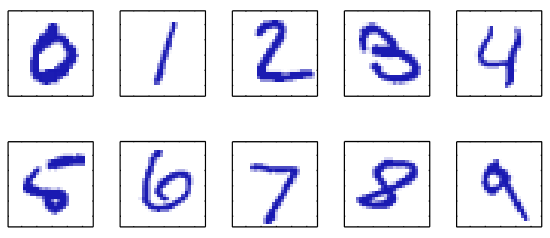
\includegraphics[width=.5\linewidth]{images/numeroClassificacao.png}
    \source{\citeonline{machineLearning}}
\end{figure}

No exemplo apresentado na \autoref{fig:numeroClassi}, podemos entender a tarefa
como  um sistema  no qual  $x$ é  a entrada  e $\hat{Y}$  é conjunto  de saída.
Matematicamente,  podemos expressar  da forma  vista na  \autoref{eq:sisCla}. A
saída será na forma  de um conjunto de números variando de 0  a 1 expressando a
probabilidade  de  $x$ pertencer  à  classe  $\hat{Y}_i$  onde  $i$ é  o  valor
expressado na imagem.

\begin{equation}
    \label{eq:sisCla}
    f(x) = \hat{Y}
\end{equation}

Prever o próximo valor de uma  série pode ser realizado considerando o conjunto
de entrada  como os valores  anteriores e o de  saída os valores  previstos. Se
assemelhando  a  tarefa  de  regressão.  Como  exemplo  se  dermos  um  sistema
$f{(x_{t-1})}  = x_t$  e tendo  um conjunto  de $n$  observações anteriores,  é
possível obter um modelo com base na identificação de padrões encontrados nesse
conjunto.

Na próxima subseção é detalhado um modelo específico de aprendizado de máquina,
as redes neurais  artificiais. Tal modelo, bem como as  técnicas de aprendizado
utilizadas, será  abordado com  foco no tratamento  de problemas  de regressão,
visto que esse é o tipo de problema tratado neste trabalho.

\subsection{Redes Neurais artificiais}

Segundo  \citeonline{haykin2009}, a  pesquisa  em redes  neurais artificiais  é
motivada pelo entendimento  de que o cérebro humano realiza  o processamento de
uma forma completamente diferente dos computadores convencionais. Essa forma de
processamento  realizado  pelo  cérebro  é altamente  complexa,  não  linear  e
altamente  paralela. A  unidade de  processamento  e organização  básica de  um
cérebro são  os neurônios.  O autor  ainda lhe  confere superior  capacidade na
realização de  tarefas como  reconhecimento de padrões  do que  os computadores
digitais.

Os animais nascem  com estruturas cerebrais que lhe serão  úteis durante toda a
vida. Apesar disso, muitas outras estruturas  se desenvolverão ao longo da vida
do individuo.  O cérebro é  concebido de maneira  muito plástica, ou  seja, ele
possui a capacidade de,  na fase de aprendizado, se adaptar  ao contexto em que
vai se  desenvolver. Esse mesmo  conceito de plasticidade também  foi utilizado
para a modelagem de redes neurais artificiais~\cite{haykin2009}.

\subsubsection{\textit{Perceptron}}

Como já colocado, assim como o  cérebro, as redes neurais artificiais possuem o
neurônio como elemento  de processamento. Um modelo de neurônio  usado em redes
artificiais é  o \textit{perceptron}. Descrito primeiramente  por Rosenblatt em
1962, tem sua  função definida pela \autoref{eq:perceptron}, sendo  dada como a
soma ponderada por $w_i$ das entradas $x_i$. Visualmente, o \textit{perceptron}
é representado segundo a \autoref{fig:perceptron}.

\begin{equation}\label{eq:perceptron}
    v(x) = \sum_{i=1}^{m}{w_i  x_i + b}
\end{equation}

\begin{figure}[ht]
    \centering
    \caption{Representação gráfica de um \textit{perceptron}}\label{fig:perceptron}
    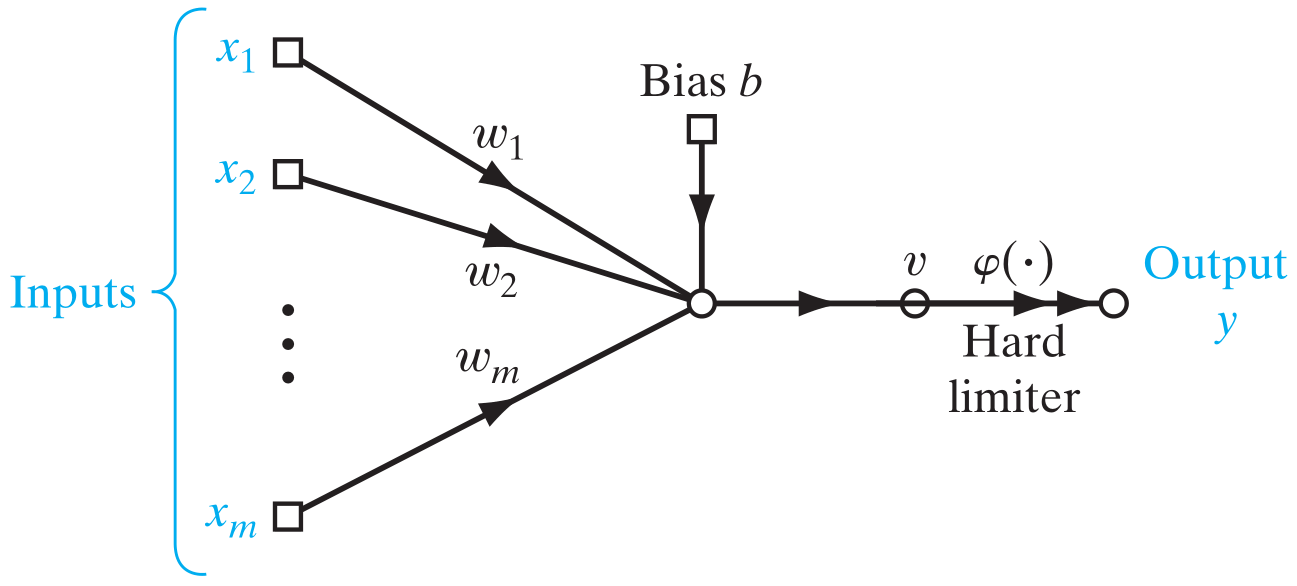
\includegraphics[width=.5\linewidth]{images/perceptron.png}
    \source{\citeonline{haykin2009}}
\end{figure}

Após  ponderação das  entradas,  é  aplicada ao  resultado  $v$  uma função  de
ativação. Classicamente, essa função é dada como uma função degrau, ou seja, se
o valor  resultante da  soma ponderada  for maior que  um valor  determinado, o
resultado  do processamento  do  neurônio  artificial é  1,  caso contrário,  é
0~\cite{knight}.

Um exemplo da função degrau é dada da forma da \autoref{eq:funLimiar}. Nesse
exemplo, a função  resulta em 1, quando o valor  do \textit{perceptron} é maior
que 0, e 0, quando menor.

\begin{equation}
    \label{eq:funLimiar}
    o(v) = \left\{
        \begin{array}{lr}
            1 & :se\  v(x) > 0\\
            0 & :se\  v(x) < 0
        \end{array}
    \right.
\end{equation}

Outras  duas  funções de  ativação  importantes  são  a  logística e  a  linear
retificada,   respectivamente,   apresentadas   em   \autoref{eq:logistica}   e
\autoref{eq:relu}. As duas  apresentam a característica de  serem continuas, no
entanto, a  função logística se limita  ao intervalo de  0 e 1, enquanto  que a
linear retificada só é limitada inferiormente em 0.

\begin{equation}
    \label{eq:relu}
    o(v) = \left\{
        \begin{array}{lr}
            v & :se\  v(x) > 0\\
            0 & :se\  v(x) < 0
        \end{array}
    \right.
\end{equation}

\begin{equation}
    \label{eq:logistica}
    o(v) = \frac{1}{1+e^{-x}}
\end{equation}

Graficamente   podemos  representar   as   funções  de   ativação  conforme   a
\autoref{fig:ativacao}.

A  função degrau  embora extremamente  simples só  tem eficacia  em tarefas  de
classificação, já que  regressões demandam dados contínuos e  esta possui saída
discretizada.

Se a aplicada  a função logística na saída é  necessário dimensionar o conjunto
de treinamento para o intervalo 0 e 1.

\begin{figure}[ht]
    \centering
    \caption{Funções de ativação}\label{fig:ativacao}
    \begin{subfigure}{.3\textwidth}
        \centering
        \caption{Função linear retificada}
        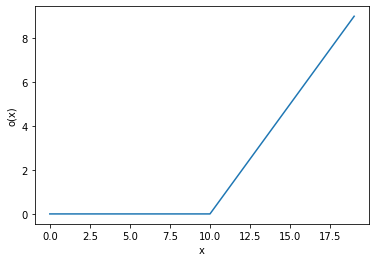
\includegraphics[width=.9\linewidth]{images/relu.png}
    \end{subfigure}
    \begin{subfigure}{.3\textwidth}
        \centering
        \caption{Função logística}
        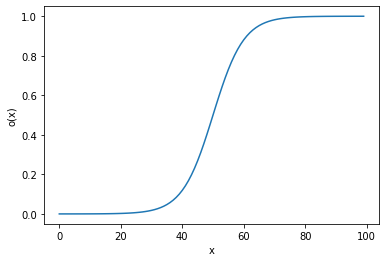
\includegraphics[width=.9\linewidth]{images/sigmoid.png}
    \end{subfigure}
    \begin{subfigure}{.3\textwidth}
        \centering
        \caption{Função degrau}
        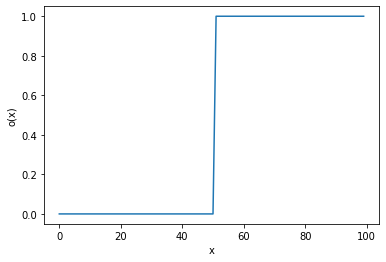
\includegraphics[width=.9\linewidth]{images/degrau.png}
    \end{subfigure}
    \source{Elaborado pelo autor}
\end{figure}

Ainda, segundo \citeonline{knight}, o  \textit{perceptron} se caracteriza pelos
pesos  e  pela  definição  da  função  de  ativação,  enquanto  o  processo  de
aprendizagem se caracteriza pela modificação desses pesos.

Porém, a  utilização de sistemas  simples com somente um  \textit{perceptron} é
insuficiente  na  solução  de muitos  problemas.  Segundo  \citeonline{knight},
o  \textit{perceptron}   sozinho  é   incapaz  de  encontrar   hiperplanos  que
resolvam problemas  de classificação não  lineares. No exemplo  apresentado por
\citeonline{knight}, é demonstrado que, enquanto um \textit{perceptron} é capaz
de reproduzir corretamente o comportamento de um  porta logica E ou OU, o mesmo
não  consegue aprender  o  comportamento  de uma  porta  OU-exclusivo. Isso  se
deve  ao limite  do \textit{perceptron}  resolver apenas  problemas linearmente
separáveis.

\subsubsection{Redes neurais \textit{feedforward}}

Embora um \textit{perceptron}  sozinho seja incapaz de  modelar algumas classes
de problemas,  eles são  capazes de  aproximar qualquer  tipo de  função quando
combinados em camadas \citeonline{knight}. A essa arquitetura de organização de
neurônios  se  dá o  nome  de  redes neurais  de  múltiplas  camadas. Quando  a
alimentação dela é na direção da  entrada para a saída será classificada também
como \textit{feedforward}.

Uma rede  neural de múltiplas  camadas pode ser  entendida como um  conjunto de
três  partes essenciais:  a camada  de entrada,  a escondida  e, por  último, a
camada de saída. A camada de entrada  é aquela que recebe as características do
conjunto de  dados. O  nome \textit{feedforward}  é dado  devido à  entrada ser
apresentada, primeiramente,  a camada de entrada  e as ativações fluírem  até a
camada de saída.  Logo, o resultado da  rede é dado pela camada  de saída, após
passar por toda  a rede em uma única direção.  Visualmente, pode-se expressar a
rede de múltiplas camadas segundo a \autoref{fig:neuralNetwork}.

\begin{figure}[ht]
    \centering
    \caption{Representação da ligação entre \textit{perceptron} em uma rede
    neural}\label{fig:neuralNetwork}
    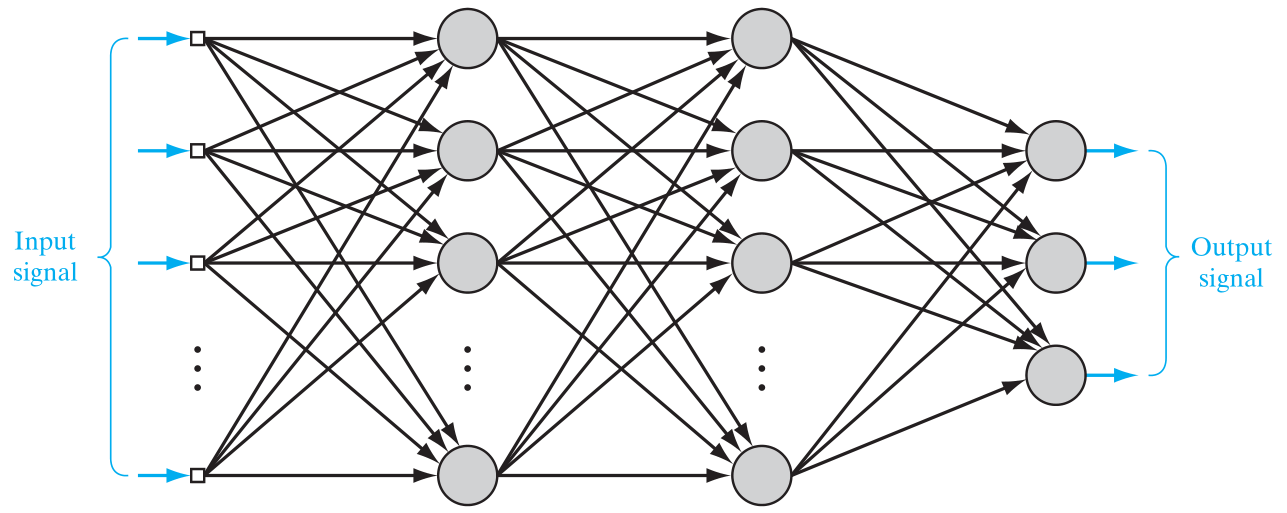
\includegraphics[width=.5\linewidth]{images/neuralNetwork.png}
    \source{\citeonline{haykin2009}}
\end{figure}

Em uma  rede neural, os  parâmetros a serem aprendidos  são os pesos  $w_i$ das
conexões entre  os neurônios das  diferentes camadas.  É comum que  esses pesos
sejam inicializados como  valores aleatórios pequenos, que  serão ajustados por
correção de erro para cada exemplo apresentado à rede.

O erro calculado na  camada de saída é dado por uma função  de cálculo do erro.
No caso de problemas de regressão, o cálculo do erro é dado pela função de erro
quadrado médio, conforme  a \autoref{eq:mse}, na qual $Y$  corresponde ao valor
real de treinamento,  $\hat{Y}$ ao valor previsto e $n$  ao tamanho do conjunto
de treinamento.

\begin{equation}\label{eq:mse}
    MSE = \frac{1}{n}\sum_{i=1}^{n}{{(Y_i - \hat{Y}_i)}^2}
\end{equation}

\subsubsection{Retropropagação}

A atualização  dos pesos  de uma rede  neural ocorre a  cada iteração  sobre os
valores de entrada. Assim, suas saídas são  comparadas com os valores reais e é
computado o  valor do erro  de acordo  com uma função  de erro. Os  valores dos
erros  $L$  são aplicados  na  \autoref{eq:backpropagation},  na qual  $\alpha$
corresponde a uma  taxa de aprendizado que regula o  tamanho do passo utilizado
na correção  dos pesos. O  erro calculado na  camada de saída  é retropropagado
para as camadas ocultadas  até chegar na camada de entrada e  os pesos de todas
as camadas é atualizado de acordo com  erro. Dessa forma, a cada nova iteração,
os pesos da rede neural são atualizados.

\begin{equation}\label{eq:backpropagation}
    w_{n+1} = w_n - \alpha \frac{\partial L(x,w_t)}{\partial w_t}
\end{equation}

\subsubsection{Avaliação e seleção do modelo}

Após  o  treinamento da  rede  neural,  deve-se  avaliar  a sua  capacidade  de
generalização  para  dados   ainda  não  vistos.  Esse  conceito   é  dado  por
\citeonline{haykin2009} como sendo um dos  principais objetivos de um modelo de
redes neurais.

Para se avaliar a capacidade de generalização, é separada uma porção dos dados,
normalmente, em uma  proporção de 30\%. Assim, durante a  etapa de treinamento,
utiliza-se  a  porção maior  dos  dados  e, após  o  modelo  estar treinado,  é
verificada a sua qualidade  utilizando a função de erro,  definida anteriormente
na \autoref{eq:mse}, mas agora no conjunto de teste (porção menor dos dados).

Já  que, durante  a etapa  de  aprendizado, o  modelo só  obtém informações  do
conjunto de treinamento, faz-se necessário algumas estratégias para impedir que
o modelo  se especialize  nesse conjunto. Essa  especialização é  conhecida por
\textit{overfit},  o  que  pode  causar  a incapacidade  do  modelo  em  prever
corretamente  os  dados  que  ainda  não  lhe  foram  apresentados.  De  acordo
com  \citeonline{deepLearning}, alguns  procedimentos podem  ser adotados  para
minimizar o \textit{overfit}, sendo eles:

\begin{enumerate}
    \item Validação cruzada\\
        O  conjunto  de  dados  é  divido  em  $k$  subconjuntos,  chamados  de
        \textit{folds},   e  a   rede  neural   é  treinada   utilizando  $k-1$
        \textit{folds}. O modelo  será validado no subconjunto  deixado de fora
        do treinamento. Ocorrerá, ainda, a mudança do conjunto que servirá para
        validação. Assim,  impede-se que a  rede se especialize em  um conjunto
        especifico. Na  \autoref{fig:crosvalidation}, o  conjunto de  entrada é
        dividido  em  três  \textit{folds}  e o  treinamento  é  realizado  nas
        três  divisões criadas,  sendo  os conjuntos  em  azul utilizados  para
        treinamento e  aqueles em  vermelho utilizados  para avaliar  o modelo.
        Essa  avaliação  ocorre  conforme  um método,  $L_{cv}$,  que  reúne  a
        avaliação de todos, $L = L_{cv}(L_1, L_2, L_3)$.

        \begin{figure}[ht]
            \centering
            \caption{Divisão da entrada em três\textit{folds}}\label{fig:crosvalidation}
            \includegraphics[width=.5\linewidth]{images/cross_validation.png}
            \source{Elaborado pelo autor}
        \end{figure}

    \item Regularização\\
        Tem como objetivo manter os pesos do modelo minimizados. O procedimento
        consiste em  alterar a função do  erro adicionando a ela  os custos dos
        pesos, conforme a \autoref{eq:regL1}. Nessa  equação, $L$ é a função de
        perda anterior e $L_{reg}$ a regularizada, $w$ são os pesos do modelo e
        $\lambda$  é  a taxa  de  regularização.  Sobre a  regularização,  cabe
        destacar  que  se  for  selecionado  um  valor  muito  alto,  os  pesos
        tenderão  a $0$  e  o  efeito prático  será  o  contrário ao  desejado.
        Consequentemente, o modelo passará a  ser incapaz de representar também
        o conjunto de entrada.

        \begin{equation}\label{eq:regL1}
            L_{reg} = L + \lambda \sum{|w|}
        \end{equation}
\end{enumerate}

Conforme  mencionado,  existem  diversos  parâmetros e  procedimentos  a  serem
considerados para  a produção do modelo  de aprendizado. A seleção  do modelo a
ser  utilizado normalmente  se dá  por  experimentação, de  forma a  selecionar
aquele que melhor  se adéque ao problema  segundo a função de  erro definida. O
procedimento de  busca pelo melhor modelo  dentro de um limite  de parâmetros é
por busca  em grade, no qual  se realiza a  indução e avaliação do  modelo para
todas as combinações de parâmetros definidas na grade.

\chapter{Trabalhos relacionados}\label{chap:trab_relacionados}

Com objetivo de entender e analisar como os modelos estudados se comportavam na
solução do problema de previsão  de séries temporais, foram analisados diversos
trabalhos.  Primeiramente, avaliou-se  os estudos  com foco  na utilização  dos
modelos  estatísticos;  em um  segundo  momento,  buscou-se por  trabalhos  que
observaram o  comportamento de modelos  de aprendizado de máquina.  Além desses
casos, também foram buscados trabalhos  que utilizaram ambos modelos em formato
de comparação, assemelhando-se assim ao objetivo deste trabalho.

% TODO: Finalizar esse trabalho relacionado

Em \citeonline{giebel2011state},  os autores utilizaram modelos  de previsão de
séries temporais para prever a geração de energia eólica, sendo a produção dada
em função da capacidade na região instalada. O vento, no entanto, é um elemento
volátil e, sendo assim, existirá momentos nos quais o uso de outras fontes será
necessária. Contudo, é preciso ter  certo conhecimento prévio, pois o ligamento
de uma usina  como aquelas movidas a  gasóleo pode levar até  duas horas. Logo,
prever duas  horas a frente pode  ser crucial para garantir  o abastecimento de
energia  para uma  região,  podendo impactar  no cotidiano  e  economia de  uma
população.

\citeonline{vinay}  utilizaram  modelos  ARIMA   e  suas  variações,  SARIMA  e
ARIMA-GARCH, para a previsão de tráfego em  rodovias. Um de seus desafios foi a
necessidade de predição em tempo real, ou seja, o modelo tinha de ser obtido ao
mesmo tempo que os dados eram  gerados. Os autores identificaram que os modelos
ARIMA tiveram  uma alta complexidade  para serem  encontrados, uma vez  que foi
adotada  uma  abordagem de  busca  em  grade  para  a identificação  do  modelo
adequado, sendo utilizada a métrica de média das somas quadradas dos erros para
avaliação.

\citeonline{reza} propuseram um modelo ARIMA modificado, acrescentando ao valor
previsto a  soma das médias dos  erros para encontrar um  modelo mais adequado.
Sua  abordagem obteve  resultados  melhores que  aqueles observados  utilizando
somente ARIMA\@.

Já no estudo  de \citeonline{matias}, o ARIMA foi comparado  com outros modelos
de base  estatística. Além disso, os  autores propuseram um modelo  híbrido. Os
modelos foram construídos para prever a demanda  de táxis na cidade de Porto em
Portugal,  com objetivo  de  melhorar  a distribuição  dos  táxis.  Um de  seus
desafios foi combinar a informação de geolocalização com as séries das demandas
por corridas. Como resultado, o modelo híbrido proposto pelos autores foi capaz
de obter um erro inferior a 26\% na previsão de corridas.

Com relação à utilização de redes  neurais para a previsão de séries temporais,
um exemplo é o trabalho de \citeonline{zhangbco}. Nesse trabalho, foi observado
o desempenho do uso de redes neurais utilizando o algoritmo de retro propagação
e  outro baseado  em algoritmos  naturais. A  série utilizada  foi a  do índice
S\&P500. Foi  comparada a  previsão entre  um e quinze  dias adiante.  O modelo
neural utilizado foi de  três camadas, com 9 neurônios na  camada de entrada, 3
na camada  escondida e  1 na camada  de saída. O  modelo proposto  utilizando o
algoritmo natural teve resultados superiores para todas as análises.

\chapter{Desenvolvimento}\label{chap:desenv}

O   desenvolvimento    deste   trabalho    foi   realizado    utilizando-se   a
linguagem   de  programação   python\footnote{\url{https://www.python.org}}  em
conjunto  com   a  plataforma  Jupyter   tanto  para  a  análise   das  séries,
quanto   para   a    produção   e   avaliação   dos    modelos   de   previsão.
Especificamente,    para    os    modelos   probabilísticos    utilizou-se    a
biblioteca   statsmodels\footnote{\url{https://www.statsmodels.org}}   e   para
os   modelos    de   aprendizado   de   máquina    utilizou-se   a   biblioteca
tensorflow\footnote{\url{https://www.tensorflow.org/}}.   Além   disso,   foram
utilizadas  as bibliotecas  seaborn, para  produção dos  gráficos, e  Pandas em
conjunto com  numpy e  scikit-learn, para importar  e realizar  as modificações
necessárias dos dados da série.

Como  colocado  na \autoref{sec:seriesTemporais},  a  capacidade  de se  prever
séries  temporais  tem  grande  importância  e  uma  de  suas  aplicações  mais
populares é na  previsão de indicadores econômicos. Desse  modo, neste trabalho
optou-se por  utilizar uma série  de caráter econômico. Um  indicador econômico
conhecido é  o S\&P500. Mantido  pela Standard \&  Poor's, o S\&P500  indexa os
valores  de  500  ativos  em  bolsas  de valores  e  serve  como  um  indicador
geral  do  comportamento do  mercado.  Os  dados  da  série podem  ser  obtidos
online\footnote{\url{https://datahub.io/core/s-and-p-500}} e  as observações do
índice  utilizadas no  desenvolvimento  deste trabalho  podem ser  visualizadas
na  \autoref{fig:sp500}. A  frequencia  dos  dados é  mensal  tendo a  primeira
observação dada em janeiro de 1871 e  ultima em abril de 2018, totalizando 1768
valores.

Para simplificar as tarefas realizadas no  decorrer deste trabalho, os dados da
série foram dimensionados no intervalo entre 0  e 1. Para isso, foi utilizado o
método \texttt{MinMaxScaler}  da biblioteca  sklearn, que  matematicamente pode
ser representado como visto na \autoref{eq:minmaxscaler}, sendo $MAX$ e $MIN$ o
intervalo  definido  para  a  série  e  $\min$  e  $\max$  funções  capazes  de
apresentar, respectivamente, o menor e o maior elemento do conjunto.

\begin{equation}
    \begin{split}\label{eq:minmaxscaler}
        &X_{std} = \frac{X - \min X}{\max X-\min X}\\
        &X_{scaled} = X_{std} * (MAX-MIN)+MIN
    \end{split}
\end{equation}

\begin{figure}[ht]
    \centering
    \caption{Gráfico das observações dimensionadas do índice S\&P500}\label{fig:sp500}
    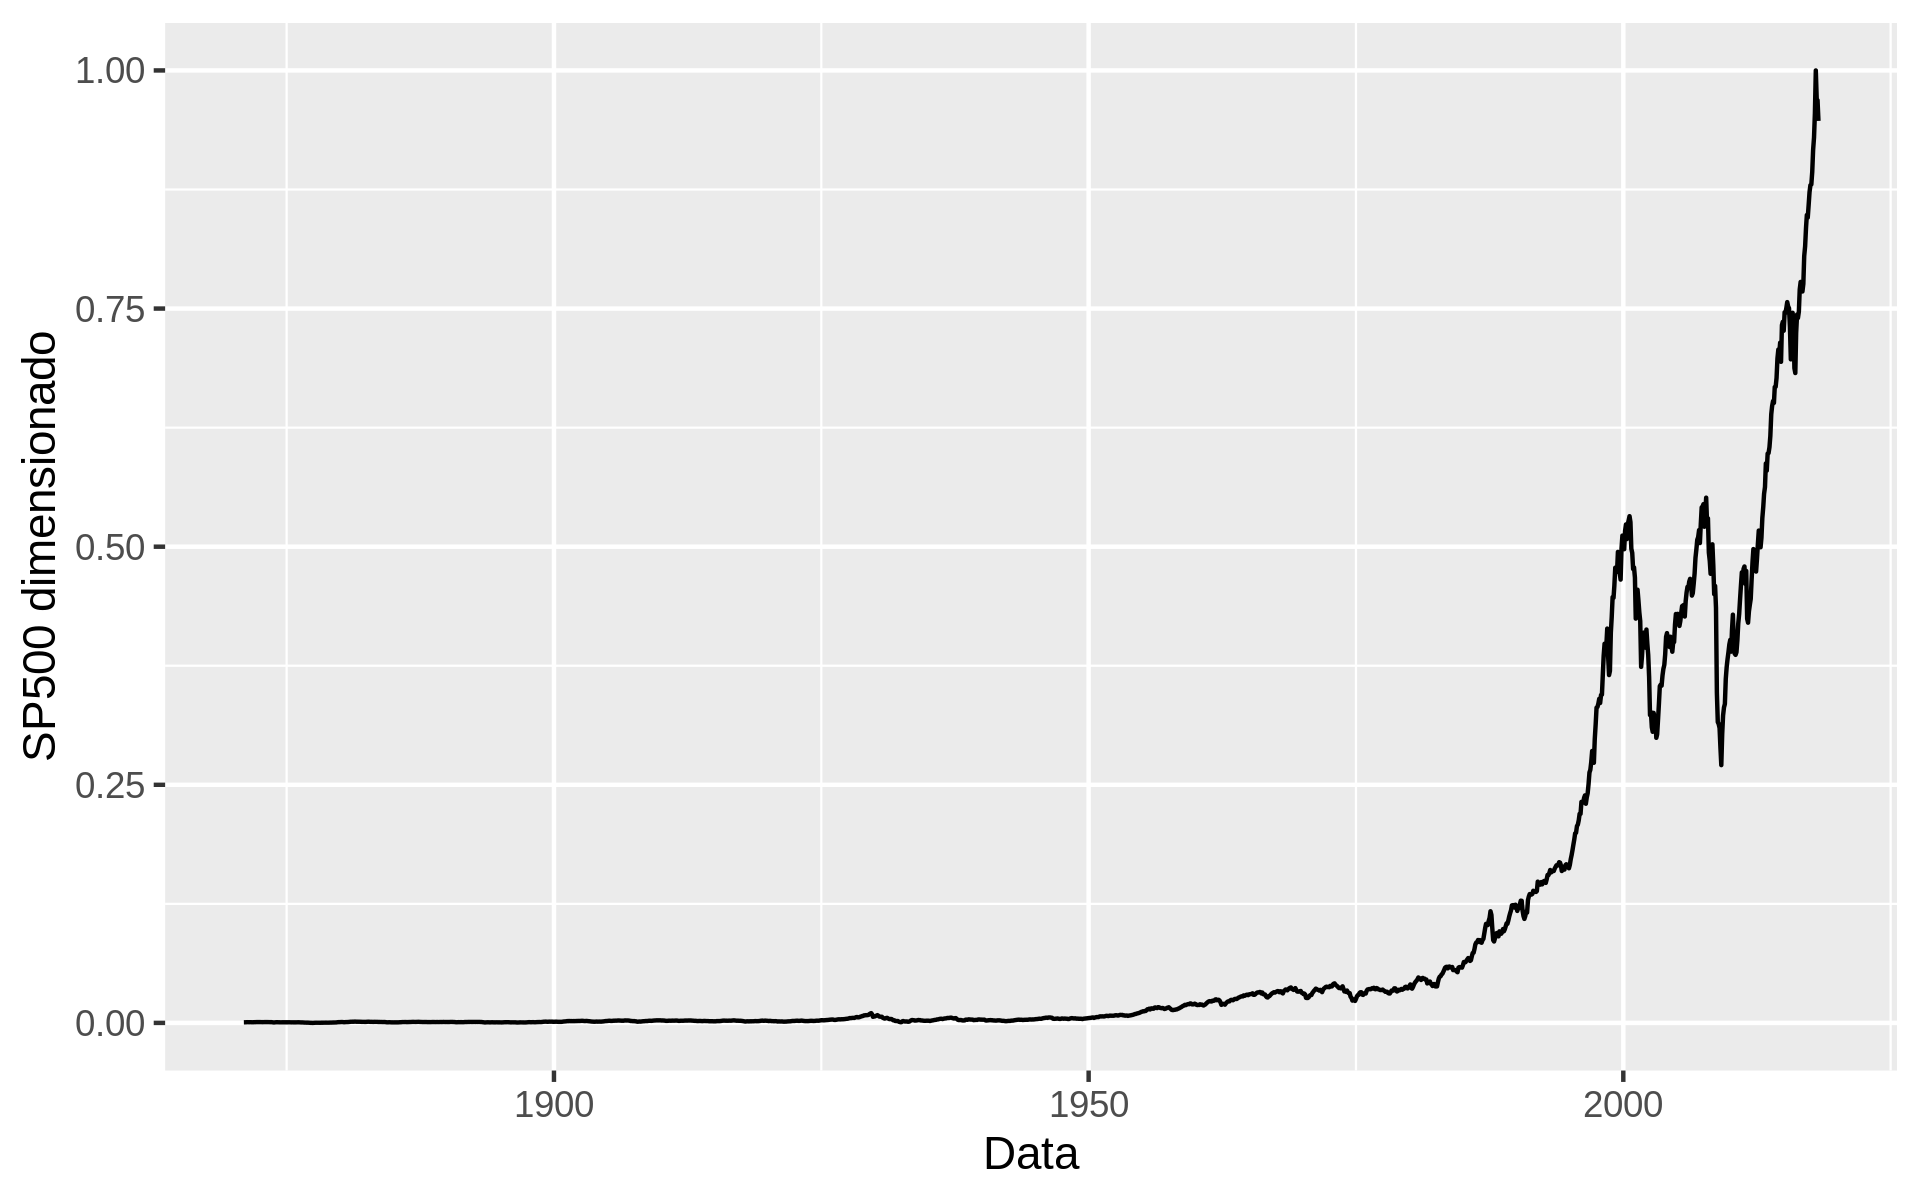
\includegraphics[width=.5\linewidth]{images/SP500.png}
    \source{Elaborado pelo autor}
\end{figure}

A  divisão dos  conjuntos de  treino  e teste  foi  realizada de  maneira a  se
utilizar 70\% dos dados para o treinamento e 30\% para a validação. Os gráficos
referentes às  observações dos  conjuntos de  treino e  teste são  mostrados na
\autoref{fig:traintest}.

\begin{figure}[ht]
    \caption{Divisão da série entre os conjuntos de treino e teste}\label{fig:traintest}
    \begin{subfigure}{.5\textwidth}
        \centering
        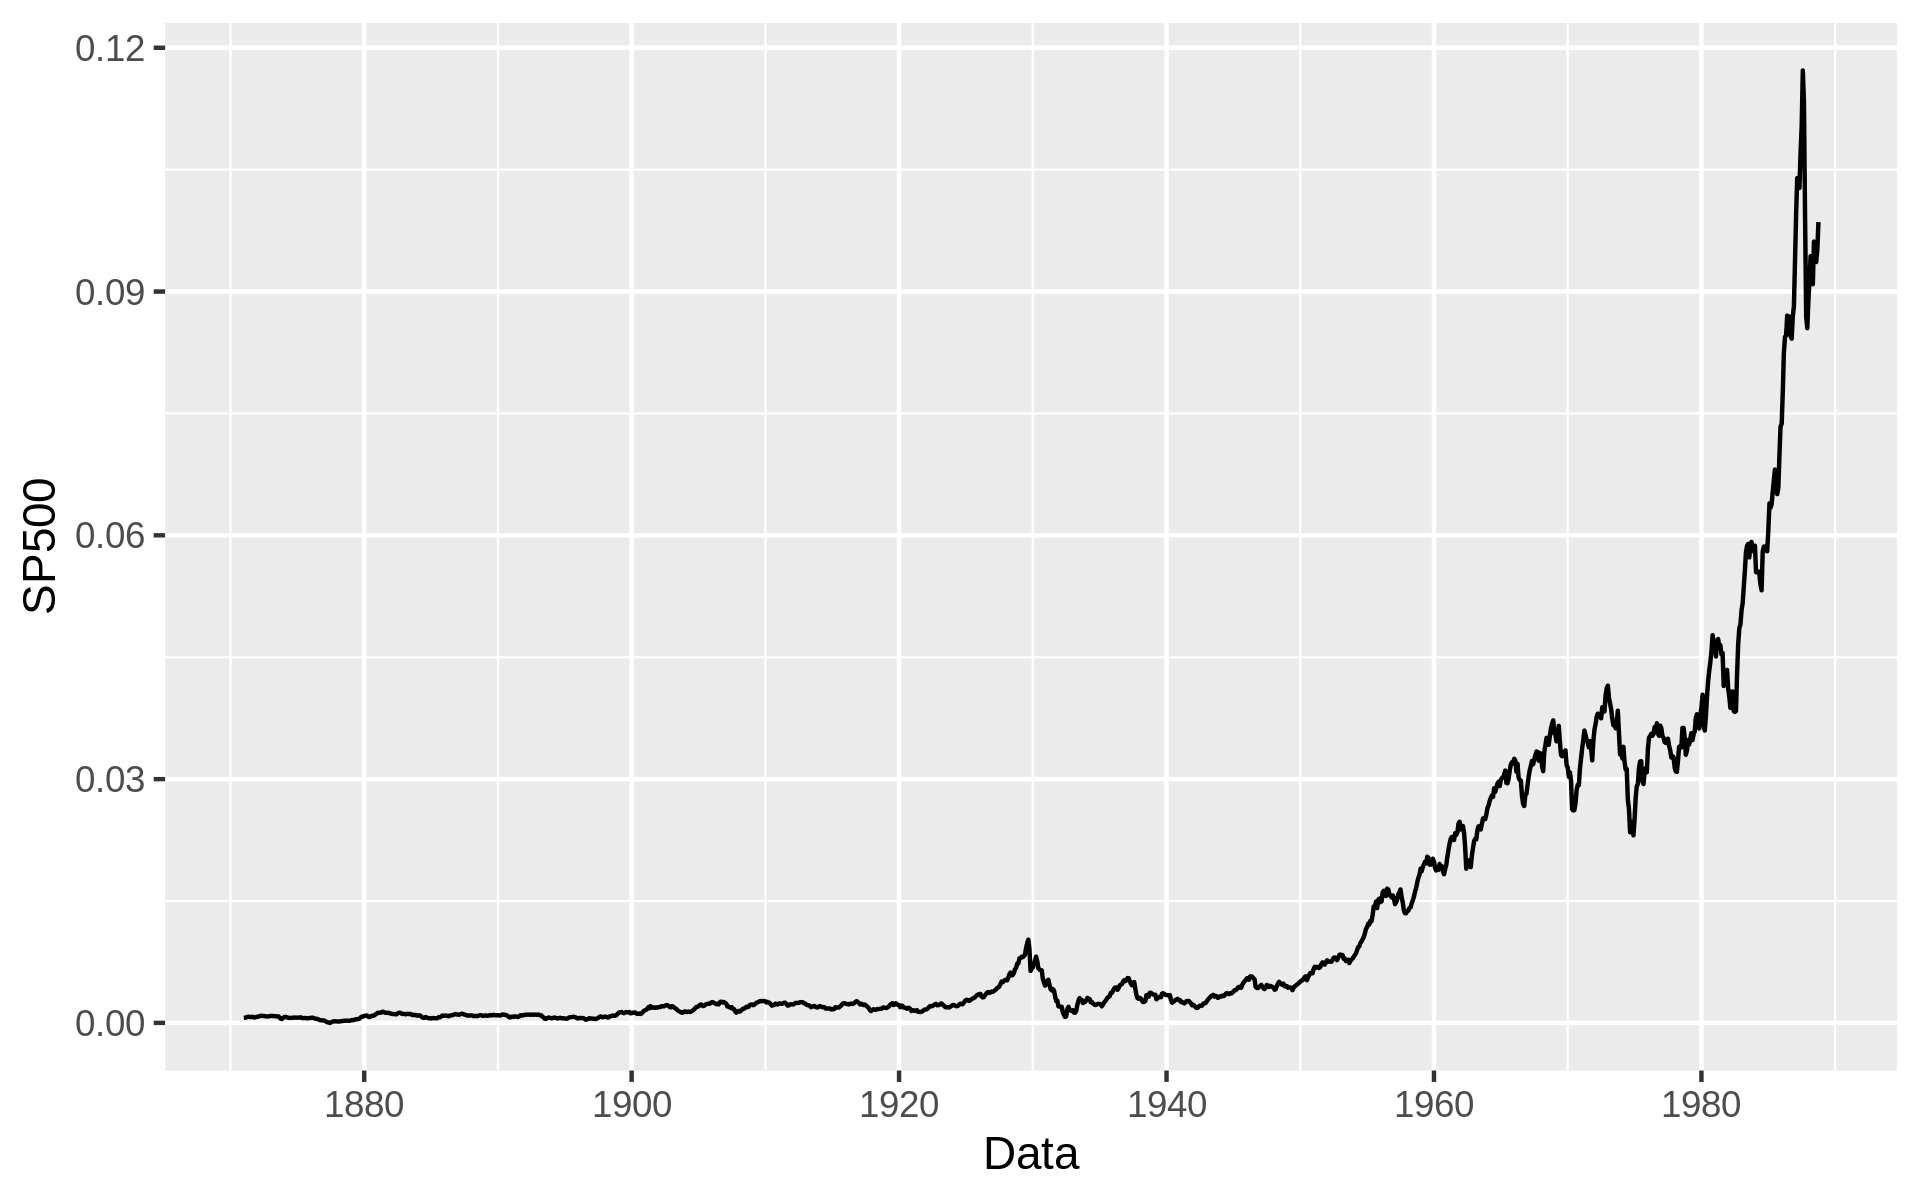
\includegraphics[width=.8\linewidth]{images/SP500_train.png}
        \caption{Conjunto de treino}
    \end{subfigure}
    \begin{subfigure}{.5\textwidth}
        \centering
        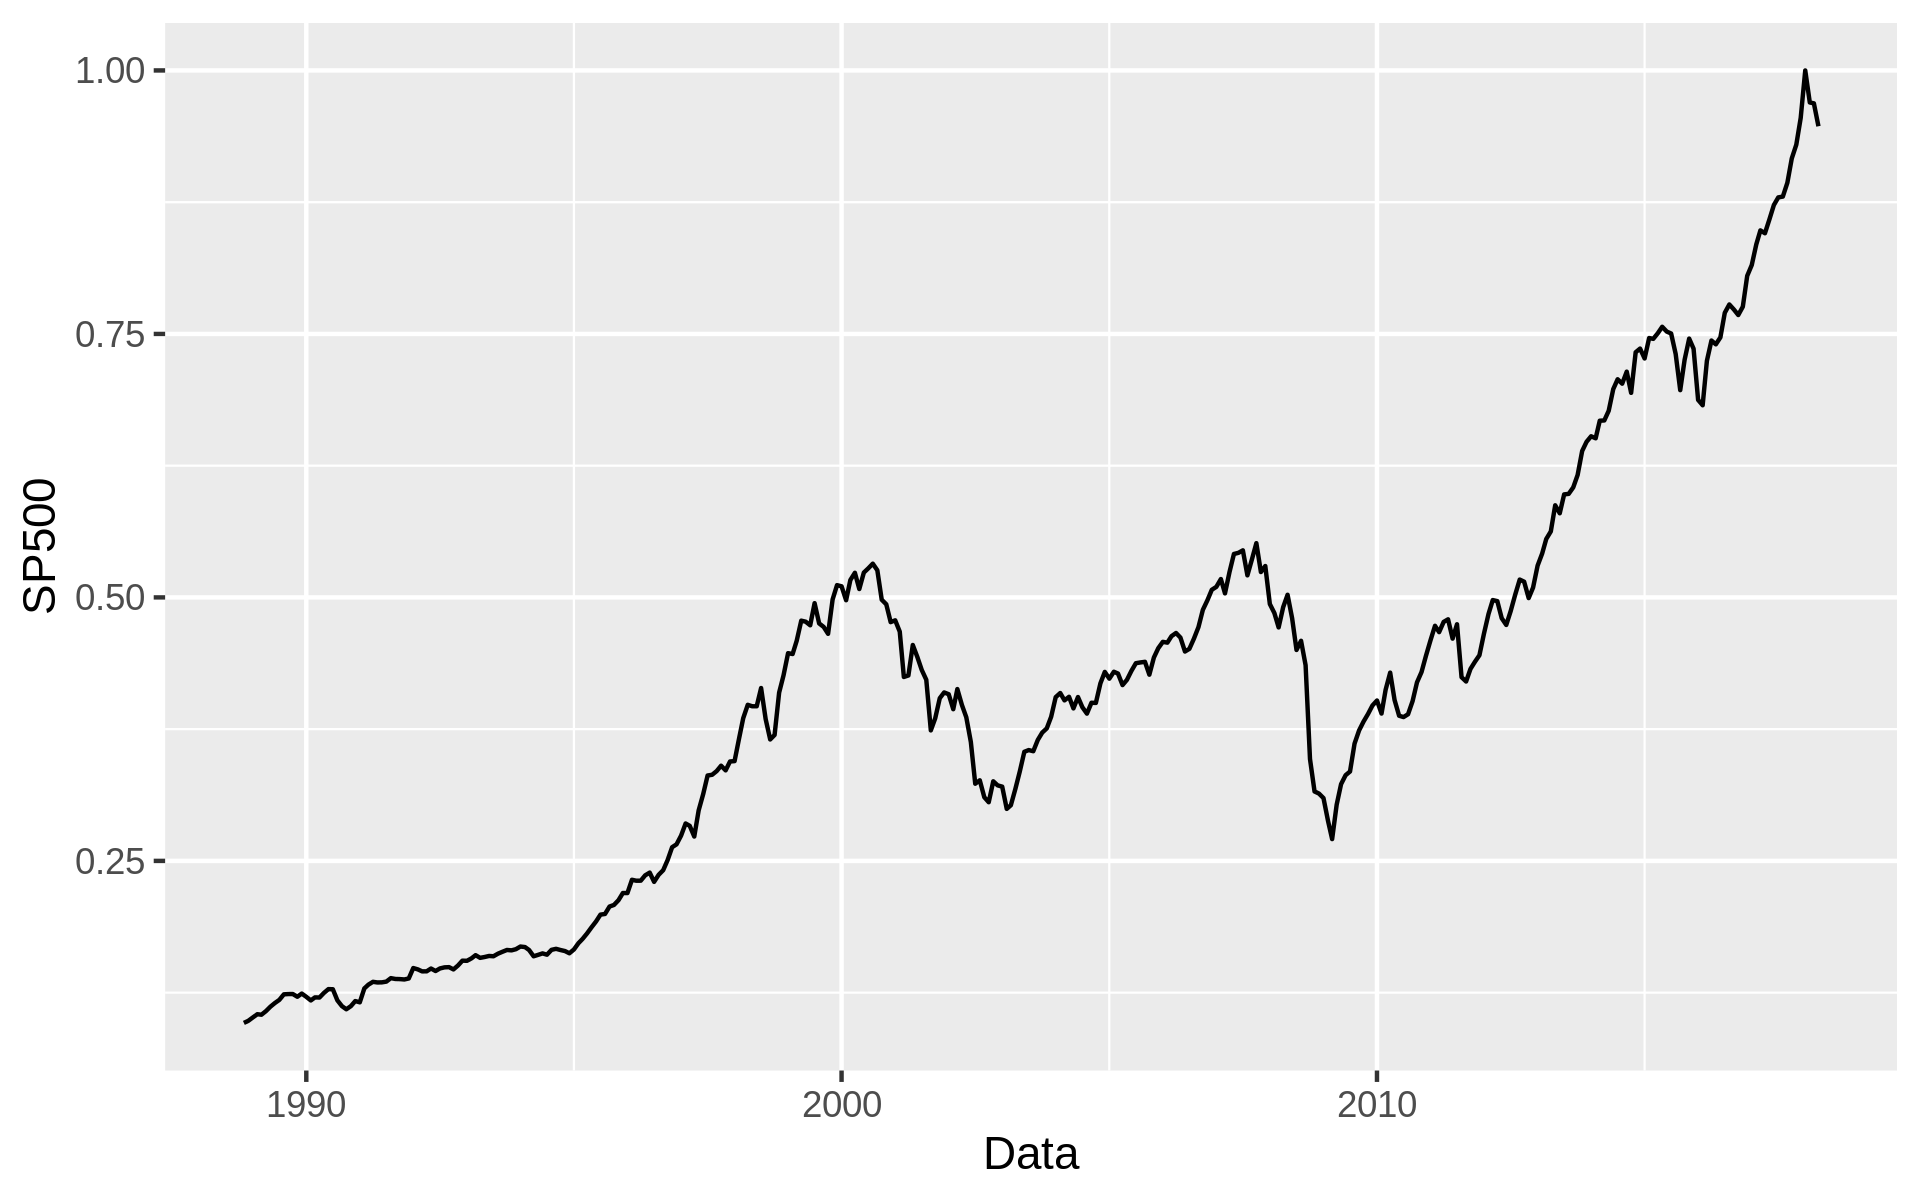
\includegraphics[width=.8\linewidth]{images/SP500_test.png}
        \caption{Conjunto de teste}
    \end{subfigure}
    \source{Elaborado pelo autor}
\end{figure}

Após a análise, foram encontrados os modelos  que mais se adéquam à série e foi
validada  a capacidade  desses modelos  prever um  dia adiante.  Para tornar  a
comparação justa, a  quantidade de observações utilizadas na  camada de entrada
do modelo de redes neurais foi igual à ordem do processo autorregressivo.

\section{Análise da série S\&P500}

Seguindo as  etapas para construção  dos modelos,  foi realizada a  análise dos
dados.  O  objetivo  era  identificar  as  características  da  série,  como  a
estacionariedade e  a possível  existência de  tendência e  sazonalidade. Nessa
etapa  também  foi  realizada  a  remoção  de  \textit{outliers}  que  poderiam
atrapalhar na construção dos modelos.

Já  no gráfico  da \autoref{fig:sp500}  percebe-se a  existência de  tendência,
permitindo  concluir que  a série  não é  estacionária. Esse  fato também  fica
evidente a  partir da análise  do gráfico da FAC  (\autoref{fig:acfsp500}), que
mostra  a existência  de  um grande  número de  correlações  positivas fora  do
intervalo de confiança.

\begin{figure}[ht]
    \centering
    \caption{Função de autocorrelação para a série S\&P500}\label{fig:acfsp500}
    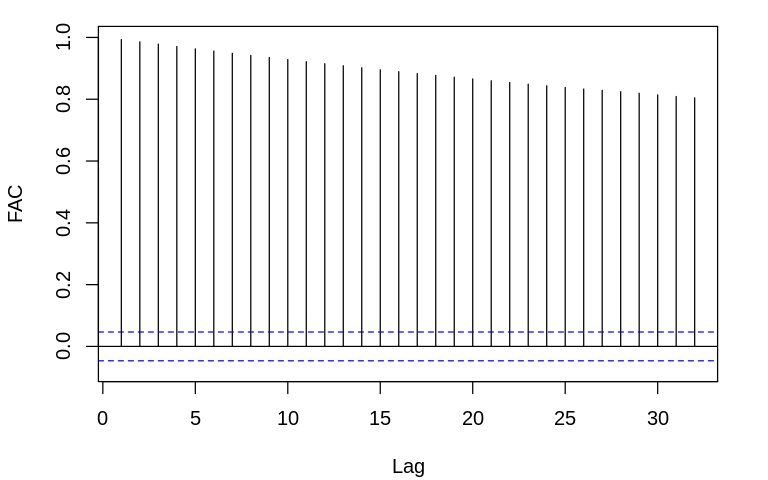
\includegraphics[width=.5\linewidth]{images/SP500_FAC.png}
    \source{Elaborado pelo autor}
\end{figure}

Para tornar a série  estacionária, inicialmente, realizou-se uma diferenciação.
A  \autoref{fig:sp500diff}  apresenta  os  dados   da  série  após  a  primeira
diferenciação. Pela observação da FAC mostrado na \autoref{fig:acf_diff_sp500},
pode-se concluir que uma única diferenciação foi suficiente para tornar a série
estacionária.

\begin{figure}[ht]
    \centering
    \caption{Primeira diferenciação dos dados do S\&P500}\label{fig:sp500diff}
    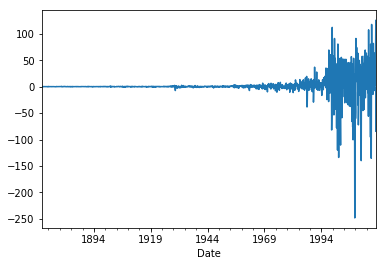
\includegraphics[width=.5\linewidth]{images/sp500diff.png}
    \source{Elaborado pelo autor}
\end{figure}

\begin{figure}[ht]
    \centering
    \caption{Função de autocorrelação da série S\&P500 diferenciada uma vez}\label{fig:acf_diff_sp500}
    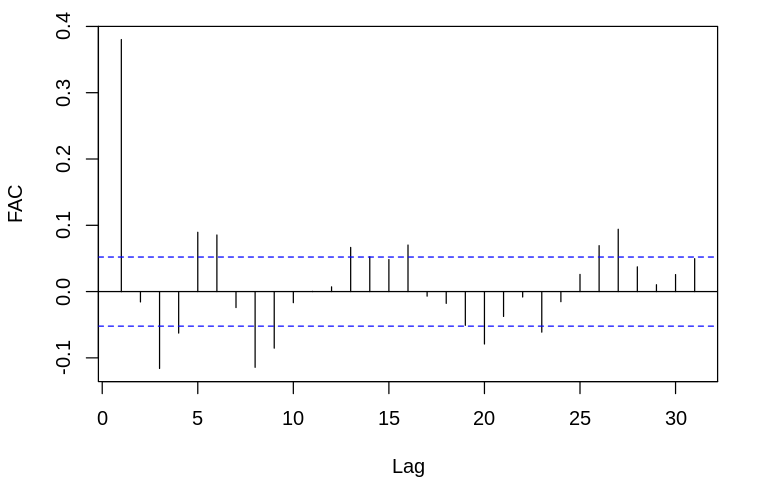
\includegraphics[width=.5\linewidth]{images/SP500_diff_FAC.png}
    \source{Elaborado pelo autor}
\end{figure}

Quanto à sazonalidade, embora seja possível observar um padrão de comportamento
na \autoref{fig:acf_diff_sp500},  não é  tão claro  qual é  o período.  Para se
definir isso, seria necessário o uso  de outras técnicas estatísticas que fogem
ao escopo deste  trabalho. Além disso, após uma diferenciação,  a série mostrou
as características necessárias para se concluir a sua estacionariedade.

Realizada da análise da série, concluiu-se que o modelo ARMA sem integração não
seria  suficiente. Assim,  o parâmetro  $d$ do  modelo ARIMA  será de  ordem 1,
devido à necessidade de uma diferenciação para tornar a série estacionária.

\section{Definição do modelo probabilístico}

Compreendido  o  comportamento  da  série, definiu-se  a  correlação  entre  as
observações para possibilitar  a construção do modelo  probabilístico. Isso foi
feito usando do  gráfico da FAC apresentado  na \autoref{fig:acf_diff_sp500} em
conjunto com o  gráfico da FACP mostrado na  \autoref{fig:sp500pacf}. Segundo o
modelo de \citeonline{box}, deve-se analisar o modelo  com $p$ sendo 1, 2 ou 5,
e para $q$ sendo 1, 2 ou 7. A seleção do melhor modelo foi dado utilizando-se o
critério de informação de Akaike (AIC).

\begin{figure}[ht]
    \centering
    \caption{Função de autocorrelação parcial da série diferenciada S\&P500}\label{fig:sp500pacf}
    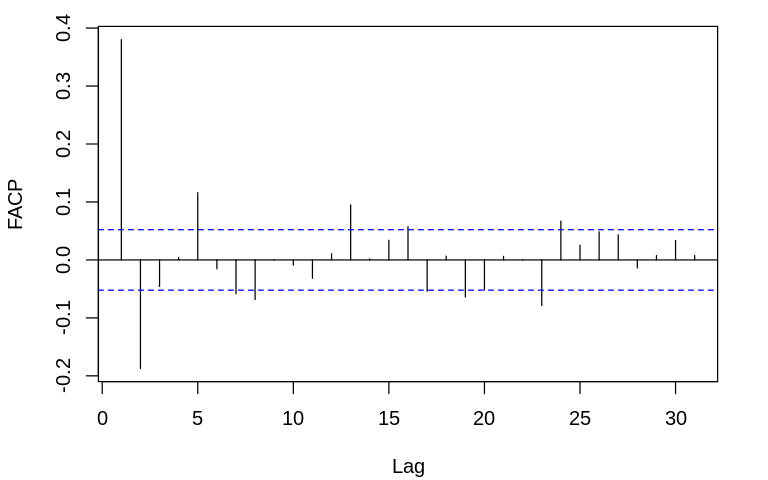
\includegraphics[width=.5\linewidth]{images/SP500_diff_FACP.png}
    \source{Elaborado pelo autor}
\end{figure}


A \autoref{tab:aicarima} apresenta as métricas AIC para os modelos propostos e,
em  destaque, o  modelo com  melhor  resultado. Como  a  AIC é  uma métrica  de
minimização,  quanto menor  o seu  valor,  melhor é  o modelo.  Logo, o  modelo
probabilístico considerado como o melhor  melhor foi o ARIMA(5,1,7), sendo esse
o modelo  utilizado para  a comparação  de desempenho com  o modelo  baseado em
aprendizado de máquina.

\begin{table}[ht]
\centering
    \caption{Valores AIC obtidos com diferentes valores de $p$ e $q$ para o modelo ARIMA($p$, 1, $q$)}\label{tab:aicarima}
\begin{tabular}{l c c c}
                        & \multicolumn{3}{c}{$q$}           \\
    $p$                 & 1      & 2      & 7               \\
    \toprule
    1                   & -15953 & -15952 & -15979          \\
    2                   & -15965 & -15968 & -15989          \\
    5                   & -15984 & -15988 & \cellcolor[HTML]{AAAAAA}\textbf{-16004} \\
\end{tabular}
\source{Elaborado pelo autor}
\end{table}

Para ser possível concluir  que o modelo é bom, deve-se,  ainda, analisar se as
funções de autocorrelação  e de autocorrelação parcial  dos resíduos apresentam
correlações significativas. Na \autoref{fig:acffigresiduals}, possível observar
que ainda  existem correlações  relevantes. No entanto,  as mesmas  são geradas
pela componente sazonal da série e, como já dito, não fizeram parte do objetivo
deste trabalho.

\begin{figure}[ht]
    \caption{Funções de autocorrelação e de autocorrelação parcial dos resíduos do
    modelo ARIMA(5,1,7) para a série S\&P500}\label{fig:acffigresiduals}
    \begin{subfigure}{.5\textwidth}
        \centering
        \caption{Função de autocorrelação dos resíduos}
        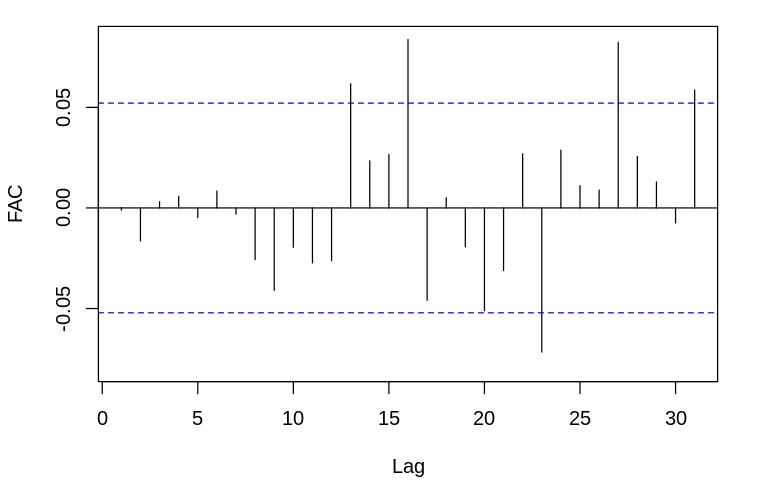
\includegraphics[width=.8\linewidth]{images/residuals_FAC.png}
    \end{subfigure}
    \begin{subfigure}{.5\textwidth}
        \centering
        \caption{Função de autocorrelação parcial dos resíduos}
        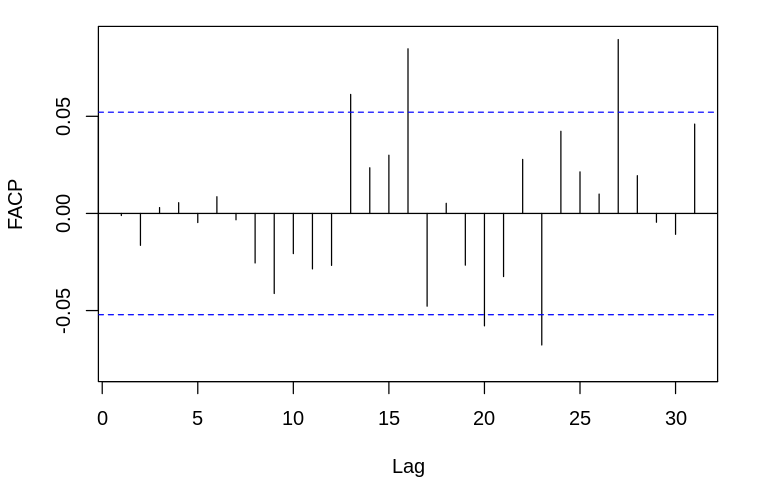
\includegraphics[width=.8\linewidth]{images/residuals_FACP.png}
    \end{subfigure}
    \source{Elaborado pelo autor}
\end{figure}

\section{Definição do modelo utilizando aprendizado de máquina}

Já para o  desenvolvimento do modelo neural, não foi  necessária uma observação
profunda da série. No entanto,  foi necessária uma parametrização mais complexa
do modelo.  Observado como o  modelo convergia e considerando-se  os parâmetros
escolhidos, foi realizada uma busca em grade extensiva para encontrar um modelo
com  melhor capacidade  de generalização.  Os parâmetros  testados na  busca em
grade são mostrados na \autoref{tab:gridsearch}.

\begin{table}[ht]
\centering
\caption{Parâmetros utilizados na busca em grade}\label{tab:gridsearch}
\begin{tabular}{l l}
\multicolumn{1}{c}{Parâmetro}        & \multicolumn{1}{c}{Possibilidades}  \\
    \toprule
    Número de camadas                & 1 \ldots 4                          \\
    Número de unidades por camada    & 1 \ldots 20                         \\
    $\lambda$ regularização          & 0.00001 \ldots 0.0001               \\
    Função de ativação               & $relu$, $sigmoid$                   \\
    Função de erro                   & MSE, MAE                            \\
    Iterações                        & 20 \ldots 500
\end{tabular}
\source{Elaborado pelo autor}
\end{table}

Uma  característica observada  nas primeiras  execuções anteriores  à aplicação
da  regularização  foi  o  rápido   \textit{overfit}  ao  conjunto  de  treino,
mesmo  com  o  uso  de  validação  cruzada,  conforme  pode  ser  observado  na
\autoref{fig:sp500_overfit}. A  aplicação da regularização foi  suficiente para
diminuir a ocorrência do \textit{overfit}.

\begin{figure}[ht]
    \centering
    \caption{Gráfico da comparação dos valores previsto e reais para o conjunto de treino e teste}\label{fig:sp500_overfit}
    \minipage{0.50\linewidth}
        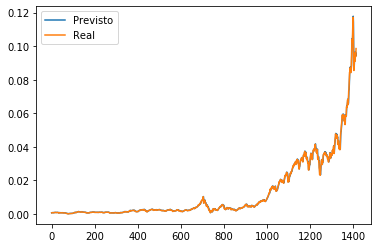
\includegraphics[width=\linewidth]{images/sp500_overfit_train.png}
    \endminipage\hfill
    \minipage{0.50\linewidth}
        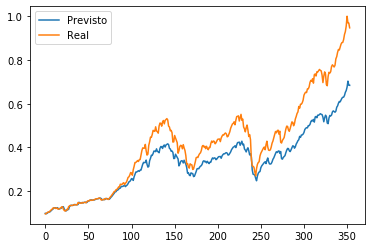
\includegraphics[width=\linewidth]{images/sp500_overfit_test.png}
    \endminipage\hfill
    \source{Elaborado pelo autor}
\end{figure}

\begin{figure}[ht]
    \centering
    \caption{Gráfico da função de erro em  função do números de iterações para
    a série S\&P500}\label{fig:iter_sp500_overfit}
    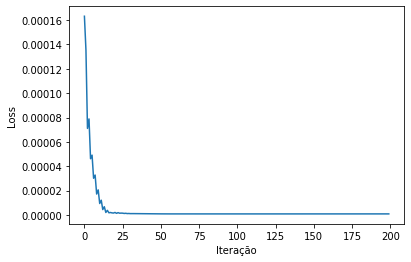
\includegraphics[width=.5\linewidth]{images/sp500_overfit_iter.png}
    \source{Elaborado pelo autor}
\end{figure}

O modelo  de redes neurais artificiais  selecionado a partir da  busca em grade
possui duas camadas.  A primeira camada possui 13 neurônios  e a segunda possui
apenas um  neurônio, já  que esta  é a camada  de saída.  A função  de ativação
escolhida  foi  a $relu$  e  o  valor  $\lambda$  da regularização  ficou  como
$0.000001$. A função de erro selecionada foi a função média dos erros quadrados
(MSE) e 300 iterações foram suficientes  para que o modelo convergisse. Uma vez
que o modelo probabilístico tem $p$ igual  a 5, foi fixado em cinco observações
a realização da previsão.

\chapter{Resultados}\label{chap:result}

A partir  dos melhores  modelos obtidos com  cada abordagem,  um probabilístico
e  um  baseado  em  rede  neural,  foram  obtidos  os  resultados  apresentados
na  \autoref{tab:resultadosp500}.  Conforme pode  ser  observado  na tabela,  a
rede neural  (MLP) apresentou  erro quadrático  médio ligeiramente  superior ao
apresentado pelo modelo ARIMA.

Conforme fica evidenciado nos gráficos mostrados na \autoref{fig:comparesp500},
os quais compara os valores previstos pelos modelos com os reais (a) e os erros
acumulados de cada modelo (b), ambos os modelos conseguiram aproximar com êxito
o  comportamento da  série.  Em  termos comparativos,  o  modelo neural  obteve
resultados um  pouco inferiores ao  modelo estatístico, uma vez  que apresentou
erros maiores, porém a diferença foi da ordem de $0,6\%$.

\begin{table}[ht]
    \centering
    \caption{Valores do erro quadrático médio para a série S\&P500}\label{tab:resultadosp500}
    \begin{tabular}{ll}
        \multicolumn{1}{c}{Modelo} & \multicolumn{1}{c}{MSE} \\
        \toprule
        MLP                        & 0,0002101               \\
        ARIMA                      & 0,0002088
    \end{tabular}
    \source{Elaborado pelo autor}
\end{table}

\begin{figure}[ht]
    \caption{Comparativos dos resultados}\label{fig:comparesp500}
    \begin{subfigure}{.5\textwidth}
        \caption{Gráfico comparativo entre os modelos obtidos}\label{fig:comprealsp500}
        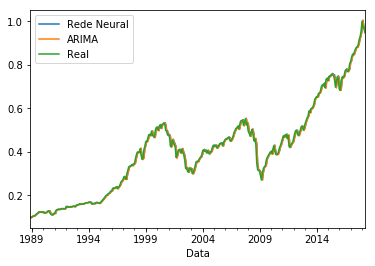
\includegraphics[width=.8\linewidth]{images/sp500_prediction_compare.png}
    \end{subfigure}
    \begin{subfigure}{.5\textwidth}
        \caption{Gráfico dos erros acumulados}\label{fig:cumsumsp500}
        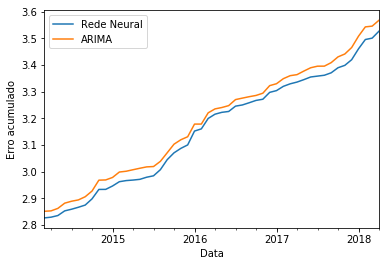
\includegraphics[width=.8\linewidth]{images/sp500_cumsum.png}
    \end{subfigure}
    \source{Elaborado pelo autor}
\end{figure}

Uma possível  explicação para  a semelhança dos  resultados pode  ser explicada
pela aparente semelhante entre um  \textit{perceptron}, utilizado em uma tarefa
de aprendizado,  e um regressor que  é base tanto do  processo autoregressivo e
do  de  médias  móveis.  Mais  claramente  ainda  se  observarmos  um  processo
autoregressivo  de  ordem 1,  dado  matematicamente  $X_t =  \alpha_1X_{t-1}  +
\epsilon_t$, é bastante semlhante a  um \textit{perceptron}, $X_t = o(X_{t-1} *
w_1 + w_0)$,  permitindo até mesmo traçar equivalências, como  os pesos da rede
neural, $w$, serem equivalentes aos coeficientes $\alpha$.

Outra  forma  que  podemos  compreender  os modelos  é  a  simplicidade  de  se
obtê-los. Para o ARIMA, foi necessária diversas observações do comportamento da
série,  e embora  não tenha  sido  o caso,  este  modelo é  muito suscetível  a
observações falhas, \textit{outliers}, que  podem demandar etapas anteriores de
pré processamento. Enquanto  que modelos utilizando redes  neurais não demandam
do usuário um grande conhecimento do comportamento ou pré processamento, já que
sua natureza  não linear é  capaz de aprender  por reconhecimento de  padrões o
comportamento  da série.  Uma  característica  inerente aos  dois  modelos é  a
complexidade do ajuste dos parâmetros, enquanto para o modelo probabilístico se
dá por da analise da serie, no modelo neural ocorre seguindo o comportamento da
etapa de aprendizado.

\chapter{Conclusões}\label{chap:concl}

O objetivo deste trabalho foi produzir e avaliar modelos preditivos para séries
temporais utilizando algoritmos estatísticos e  de aprendizado de máquina. Como
foi mostrado na  seção de Trabalhos de  Relacionados, é comum o  uso de modelos
probabilísticos, em especial o modelo híbrido ARIMA de \citeonline{box}, quando
se  realiza a  tarefa de  previsão de  séries. Mais  especificamente, o  modelo
híbrido ARIMA  proposto por \citeonline{box}.  No entanto, modelos  baseados em
algoritimos de  aprendizado de máquina  se tornaram notórios nos  últimos anos.
Logo,  neste trabalho,  foram comparados  estes modelos  para entender  as suas
capacidades e observar os seus desafios particulares.

Para  permitir a  avaliação, foi  necessária  a compreensão  da construção  dos
modelos.  O proposto  por  \citeonline{box} apresentou  uma complexidade  muito
superior na etapa  de análise da série,  já que esse modelo  pode ser entendido
como  dependente  de  diversas  intervenções  para  melhor  parametrização.  Já
o  modelo  de  aprendizado,  utilizando redes  neurais  de  múltiplas  camadas,
apresentou  uma  necessidade mínima  de  compreensão  dos dados  estudados.  No
entanto, sua complexidade se apresentou durante a etapa de treinamento.

Quanto aos resultados,  pôde-se concluir que os modelos  utilizados foram muito
similares  em  seus  desempenhos.  Vale  notar  que  os  resultados  não  foram
expressivos  na conclusão  de  superioridade  de um  modelo.  Quanto à  métrica
utilizada para a avaliação, o modelo ARIMA teve resultado superior em uma ordem
ínfima, 0,6\%, em relação ao modelo de redes neurais.

Os modelos probabilísticos  obtidos foram um modelo hibrido ARMA  de ordem 5 do
processo autorregressivo e de ordem 7  para o processo de médias móveis. Também
foi  necessária uma  diferenciação, já  que a  série apresentou  tendência. Por
conta disso,  foi necessária a  diferenciação para  para obtenção de  uma série
estacionária, característica requerida pelo modelo ARMA\@.

Para obtenção do  modelo de redes neurais,  a mudança dos dados  se resumiram a
realizar de um dimensionamento para um intervalo de valores. Sem ser necessário
maior  avaliação   do  comportamento,  já  que,   segundo  \citeonline{haykin},
algoritimos de aprendizado são ditos dirigido  por dados. No entanto, durante a
etapa  de treinamento  foi  necessária  a realização  de  diversos testes  para
encontrar  o modelo  que melhor  se adequava,  além da  aplicação de  validação
cruzada e  regularização para  diminuir a  ocorrência de  \textit{overfit}. Por
meio  desse processo,  identificou-se uma  rede neural  de duas  camadas: a  de
entrada com  13 unidades de  processamento, \textit{perceptron}, e a  segunda a
camada de  saída com  um único  neurônio, representando a  previsão um  passo a
diante.

Conclui-se, então,  que os modelos são  suficientes para a tarefa.  No entanto,
deve-se observar que os modelos  estatísticos tornam a parametrização uma etapa
muito mais  complexa que o  modelo de aprendizado.  Assim, a escolha  do modelo
pode ser feita analisando capacidade de análise de quem o constrói, ou conforme
o comportamento dos dados no caso do uso de redes neurais artificiais.

\section{Trabalhos futuros}

Um  possível trabalho  futuro é  a  avaliação de  diferentes modelos  híbridos.
Aproveitando-se  da  capacidade  dos  modelos  probabilísticos  em  representar
comportamento  linear  e,  também,  a  capacidade  de  modelos  de  aprendizado
em  séries não  lineares, como  feito por  \citeonline{oCaraLaDoModeloHibrido}.
Uma  outra possibilidade  é  a  utilização de  redes  neurais recorrentes,  que
se  diferenciam  de  modelos  \textit{feedforward}  por  possuir  memorio.  Uma
arquitetura de  redes neurais que tem  apresentado bons resultados é  a LSTM\@.
Alguns  trabalhos, como  \citeonline{oDoCaraQueComparaArimaComLSTM}, demonstram
que  é  possível  obter  resultados   superiores  com  sua  aplicação.  Podemos
ainda  estudar essas  comparações  com séries  de  comportamento diferente,  e,
consequentemente, utilizar  modelos estatísticos mais completos,  como o SARIMA
ou SARIMAX\@.

\postextual

\bibliography{referencias}

\end{document}
